% Intended LaTeX compiler: pdflatex
\documentclass[12pt]{article}
\usepackage[utf8]{inputenc}
\usepackage[T1]{fontenc}
\usepackage{graphicx}
\usepackage{grffile}
\usepackage{longtable}
\usepackage{wrapfig}
\usepackage{rotating}
\usepackage[normalem]{ulem}
\usepackage{amsmath}
\usepackage{textcomp}
\usepackage{amssymb}
\usepackage{capt-of}
\usepackage{hyperref}
\author{Liam Hurwitz}
\date{\today}
\title{Testprotokoll}
\hypersetup{
 pdfauthor={Liam Hurwitz},
 pdftitle={Test Protokoll},
 pdfkeywords={},
 pdfsubject={},
 pdfcreator={Emacs 26.3 (Org mode 9.4)}, 
 pdflang={English}}
\begin{document}

\maketitle
\newpage
\tableofcontents

\newpage
\section{Einleitung}
Dieses Testprotokoll basiert auf der C4 Testabdeckung, dann versuchen wir jede Variante unserer Software zu testen. Falls nicht anders aufgeschrieben, ist anzunehmen, dass die Tests die erwarteten Ergebnisse hatten. 

\section{Login Screen}
\label{sec:orgc5dc561}
\subsection{Registrierung}
Tested succesfully by Santiago on 02.08\\\\
Auf diesem Bildschirm kann sich der Benutzer anmelden, dazu ist es notwendig, dass der User einen Namen und ein Passwort eingibt.\\
Eingabe: Karsten als Username und Hoelscher als Passwort.\\
Ergebnis: Registrierung ist erfolgreich. Der Spieler kann sich nun einloggen.\\
\begin{figure}[htp]
\centering
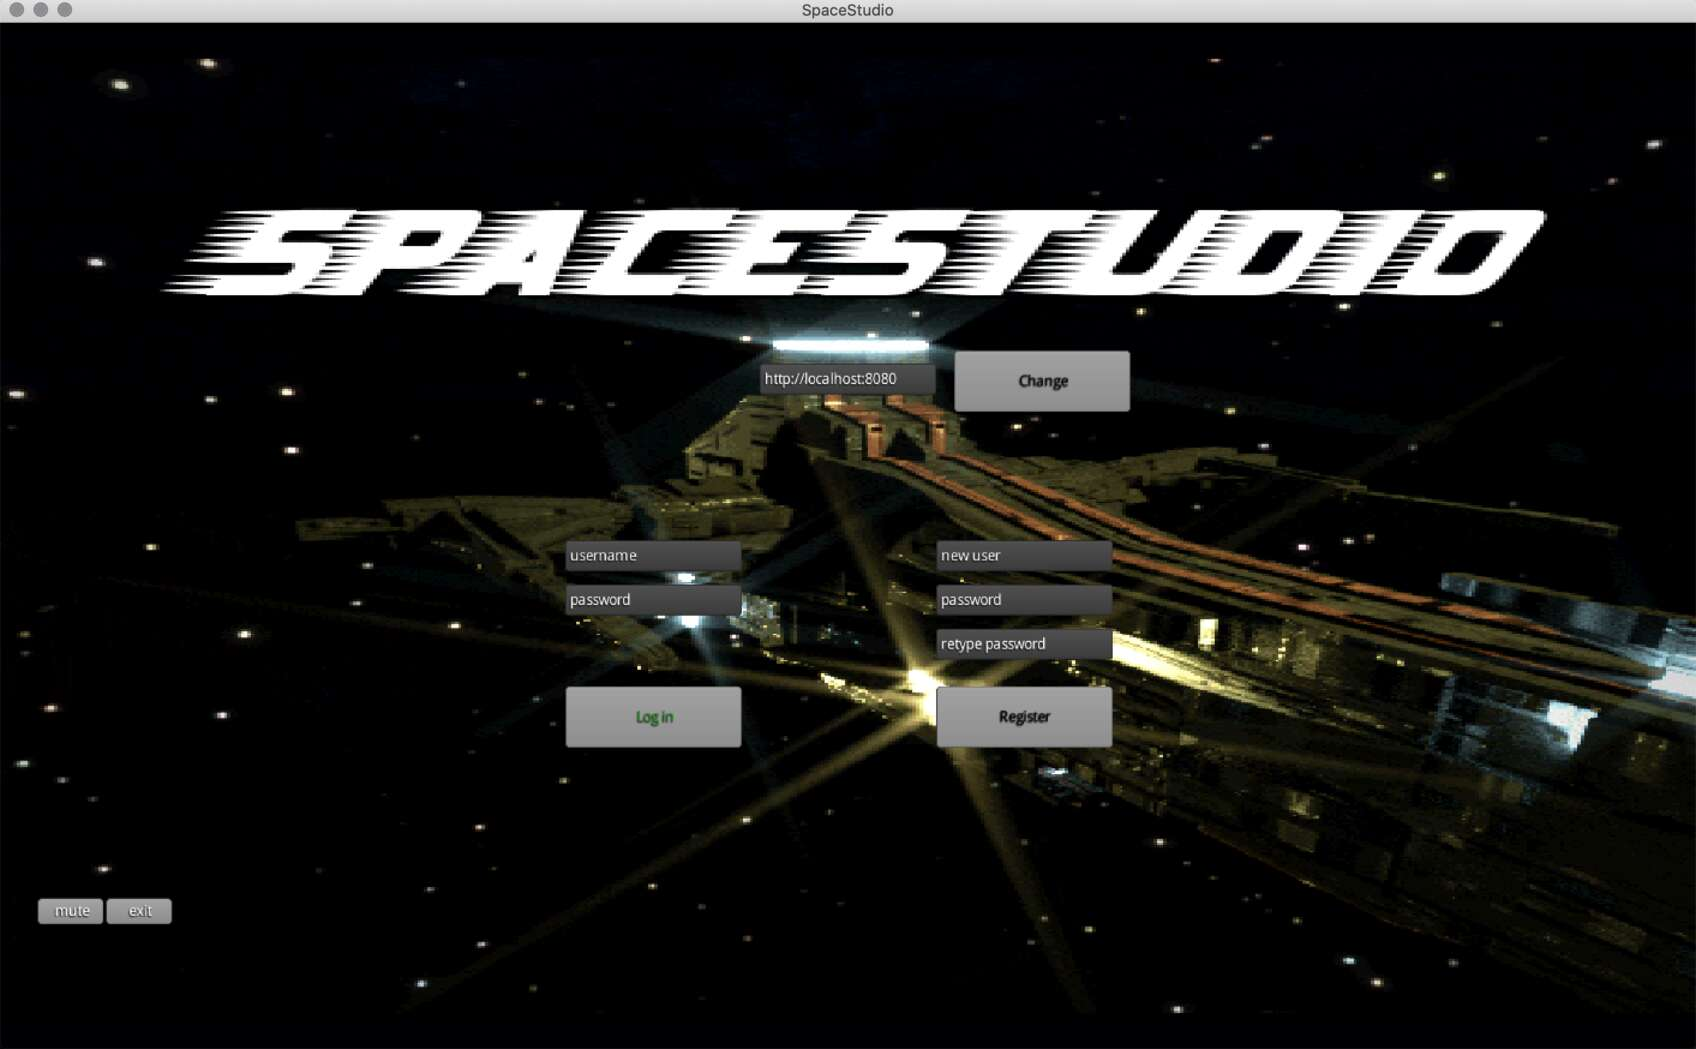
\includegraphics[scale=0.4]{TestProtocolBilder/startScreen.jpg}
\caption{Start Screen}
\end{figure}

\newpage
\subsubsection{Erfolgreiche/Fehlerhafte  Registrierung}
Tested succesfully by Santiago on 02.08\\\\
Wenn der Benutzer die Felder korrekt eingegeben hat, erhält er eine grüne Rückmeldung, in der sich die Bestätigungsnachricht des Servers für die Erstellung seiner Instanz befindet. Korrekt bedeutet es gibt das Username noch nicht und das Passwort ist in beiden Passwort-Feldern identisch.\\
\begin{figure}[h]
\centering
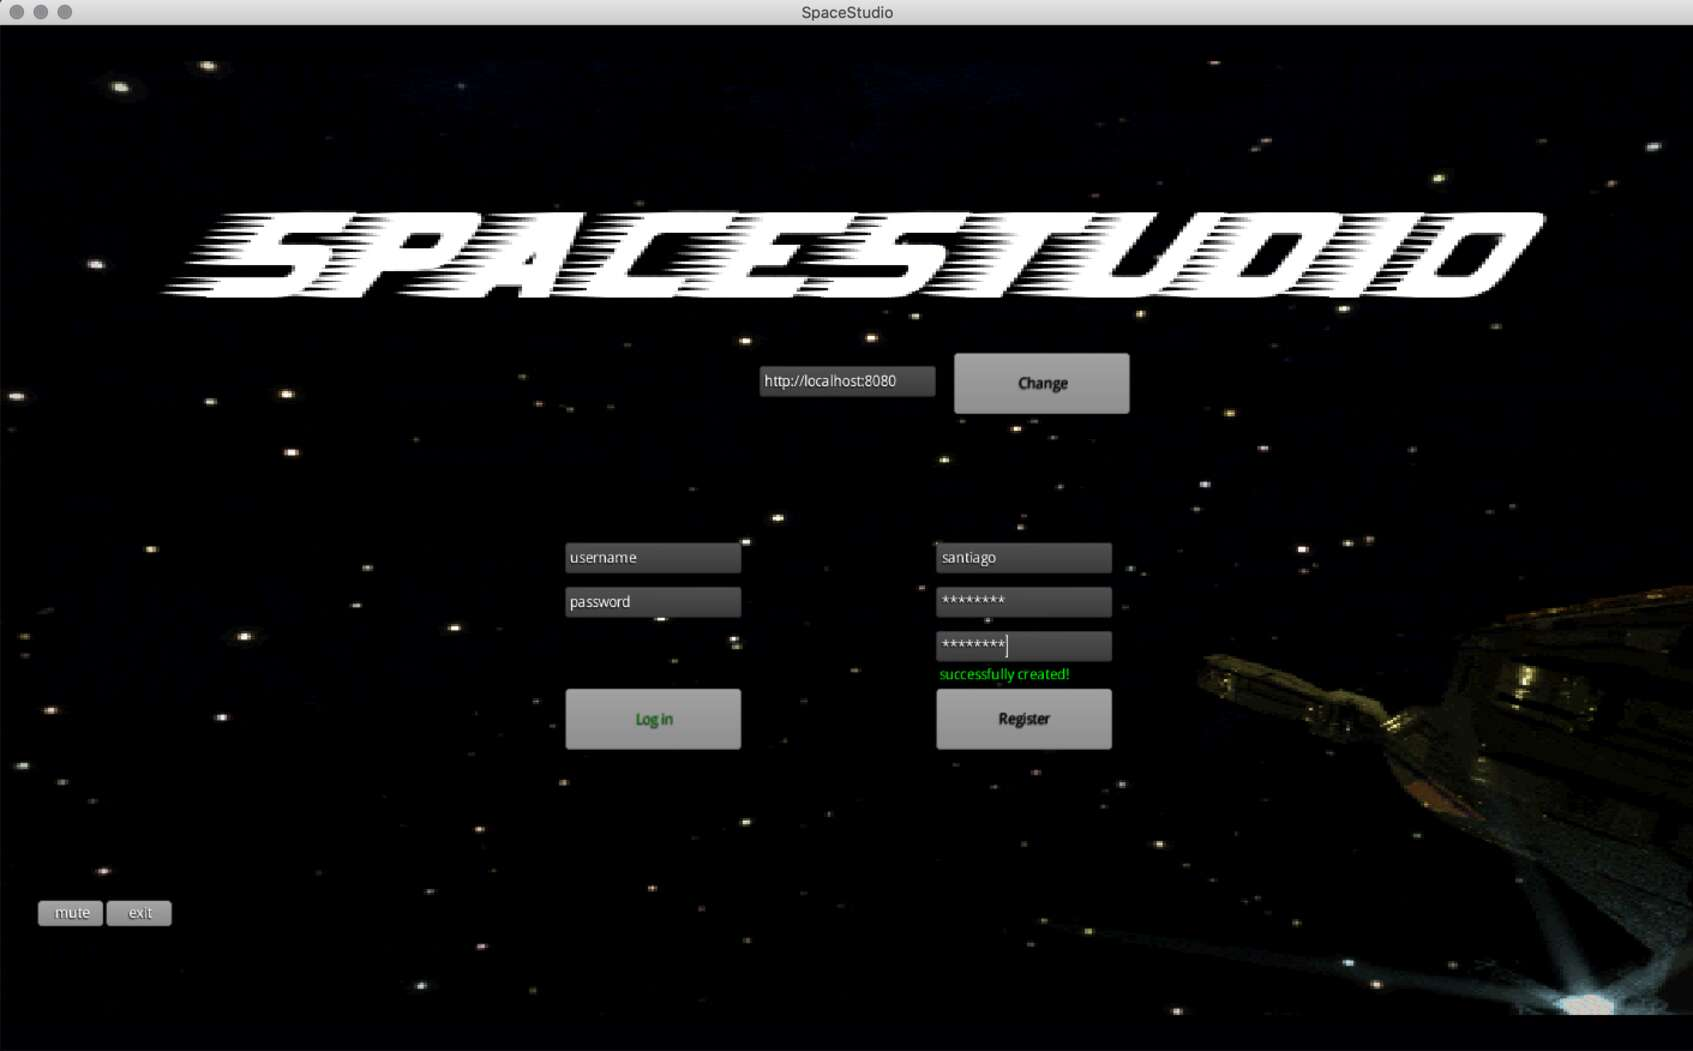
\includegraphics[scale=0.4]{TestProtocolBilder/erfolgAnmelden.jpg}
\caption{Erfolg Anmelden}
\end{figure}

Wenn der Benutzer fehlerhafte, bereits vorhandene oder unvollständige Daten in die Registrierungsfelder schreibt, erhält er eine negative Rückmeldung, in der das Problem dargestellt wird, auf das der Server beim Speichern der Daten gestoßen ist.\\
\begin{figure}[h]
\centering
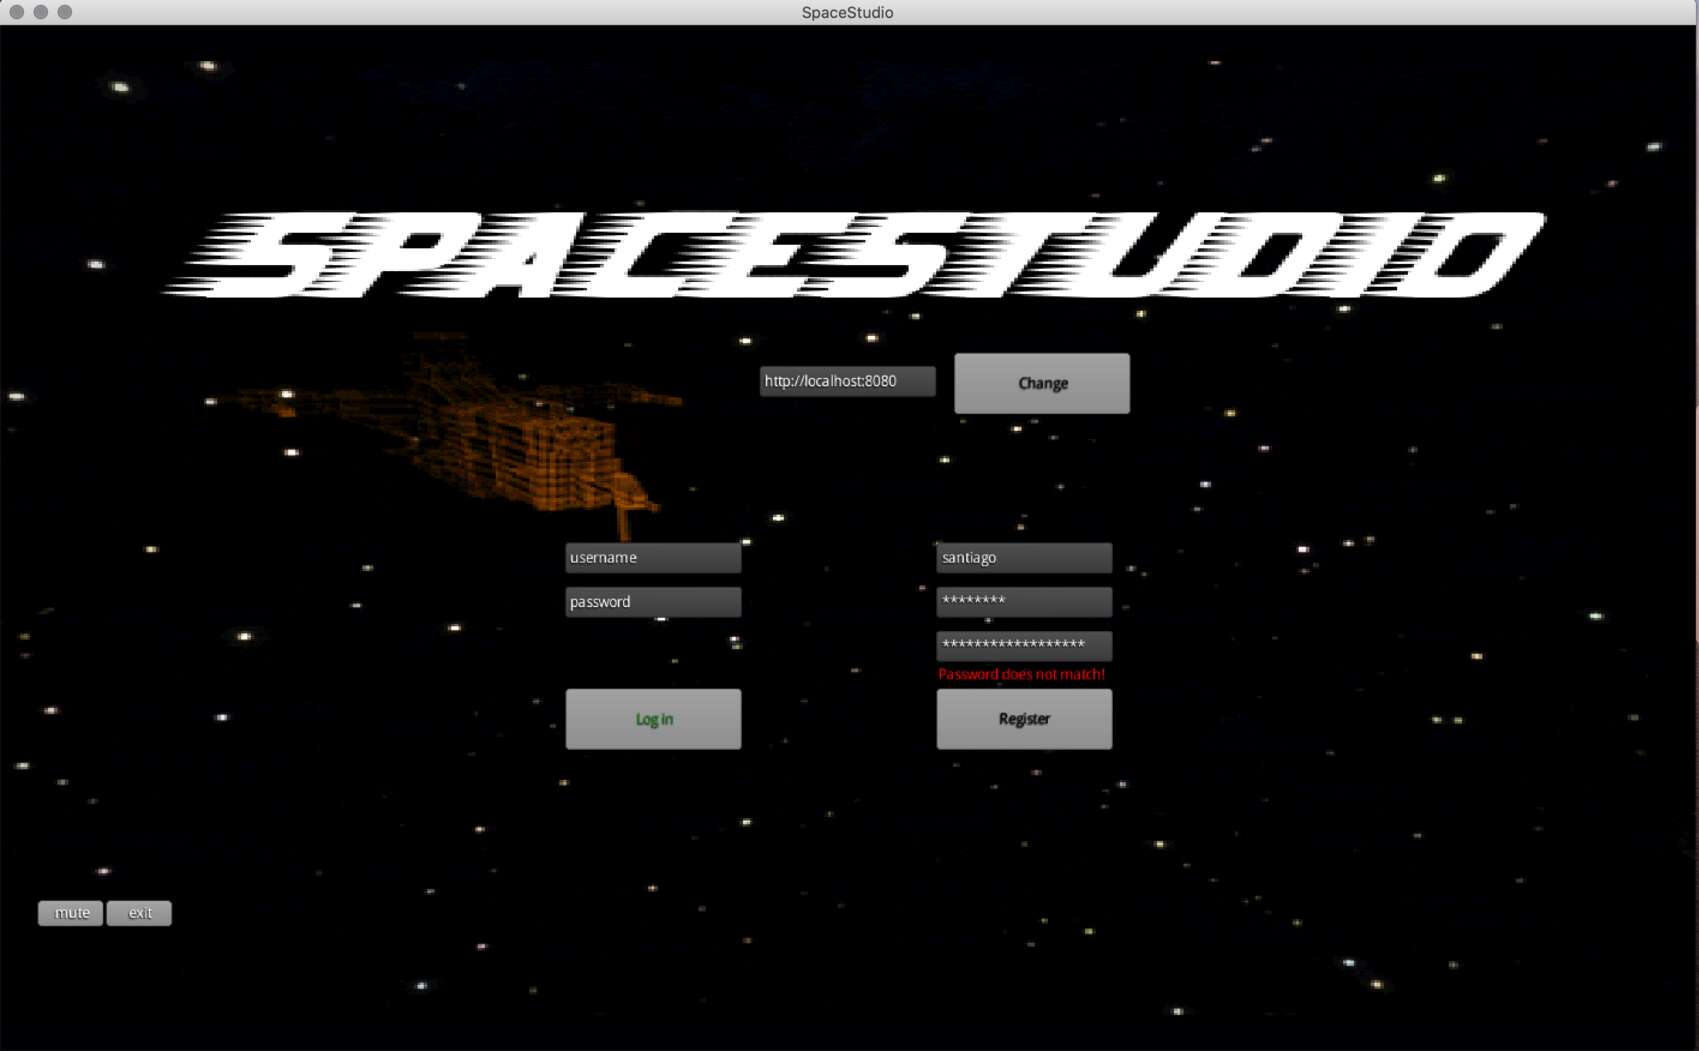
\includegraphics[scale=0.4]{TestProtocolBilder/doesnotMatchPassword.jpg}
\caption{Ungültiger Name oder Passwort}
\end{figure}
\newpage
\subsubsection{Erfolgreiche Registrierung}
Tested succesfully by Santiago Rey on 02.08\\\\
Wenn sich der Benutzer mit gültigem Namen und Passwort registriert hat, überprüft der Server die Daten und speichert diese in der Datenbank.\\

\begin{figure}[h]
\centering
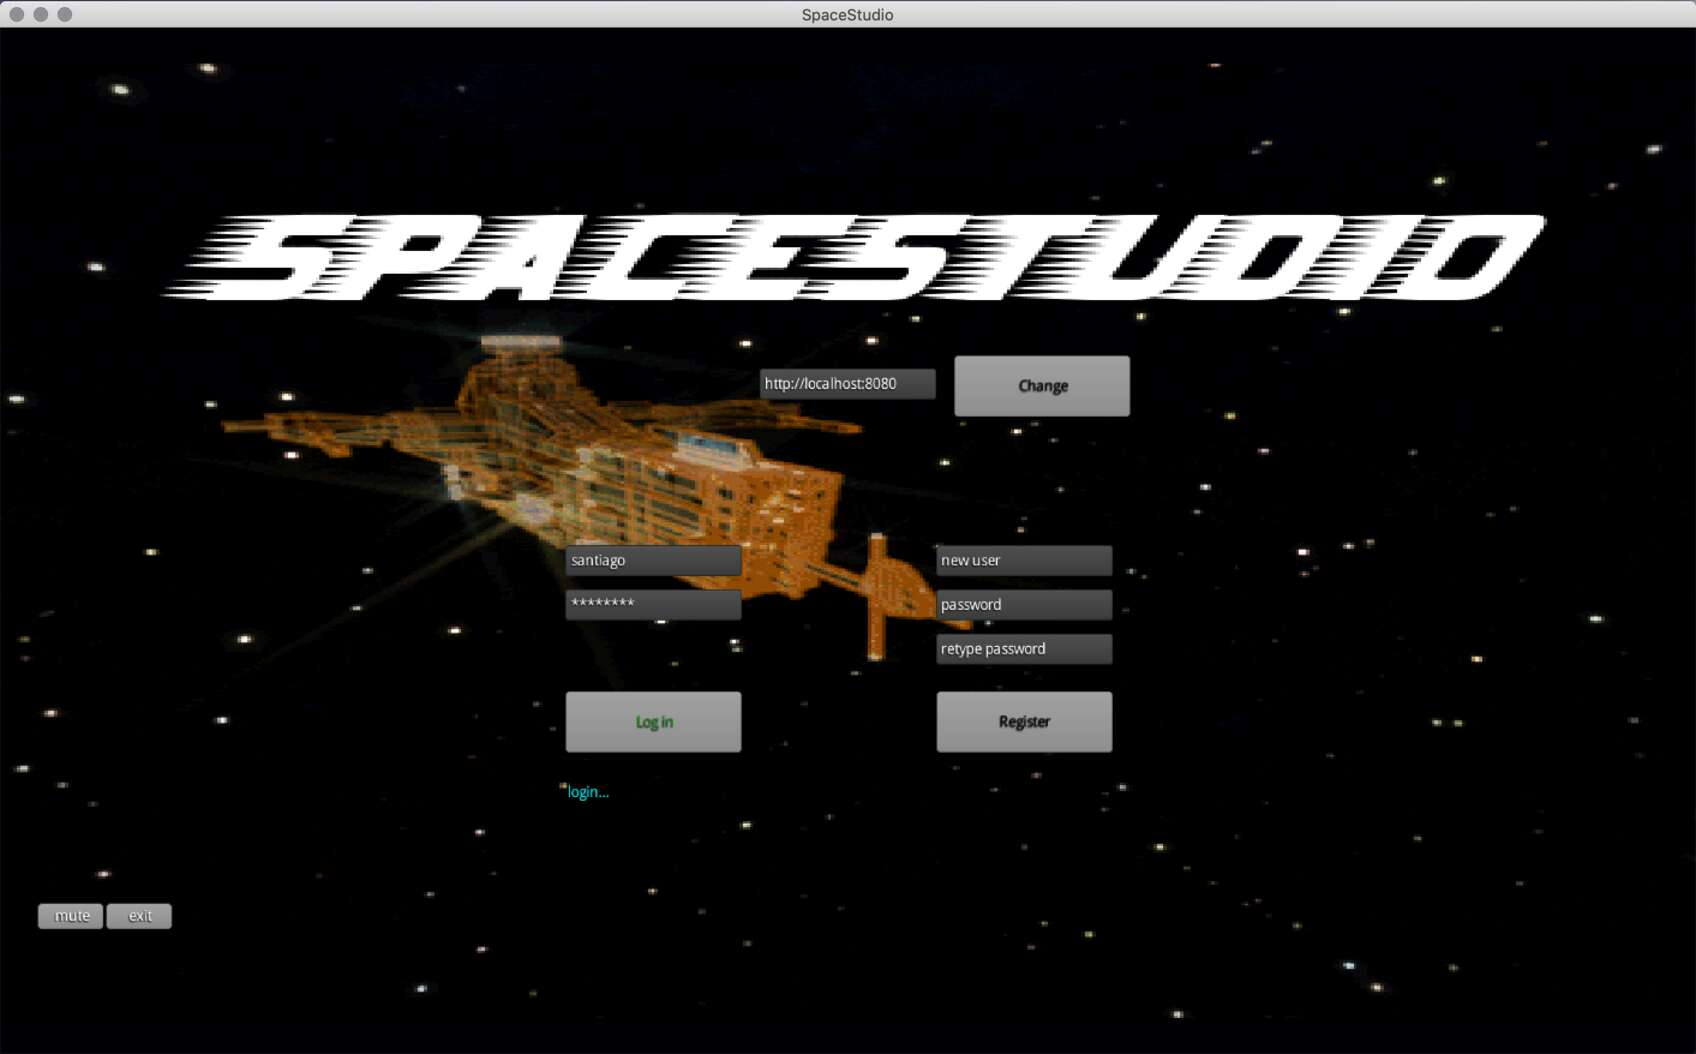
\includegraphics[scale=0.4]{TestProtocolBilder/erfolgLogin.jpg}
\caption{Login Erfolg}
\end{figure}
\newpage
\subsection{Anmeldung}
\subsubsection{Fehlerhafte Anmeldung}
Tested succesfully by Santiago Rey on 02.08\\\\
Wenn sich der Benutzer mit ungültigen Daten versucht anzumelden, kann der Server den Benutzer nicht validieren, sodass er nicht zum nächsten Bildschirm weitergeleitet werden kann.
\begin{figure}[h]
\centering
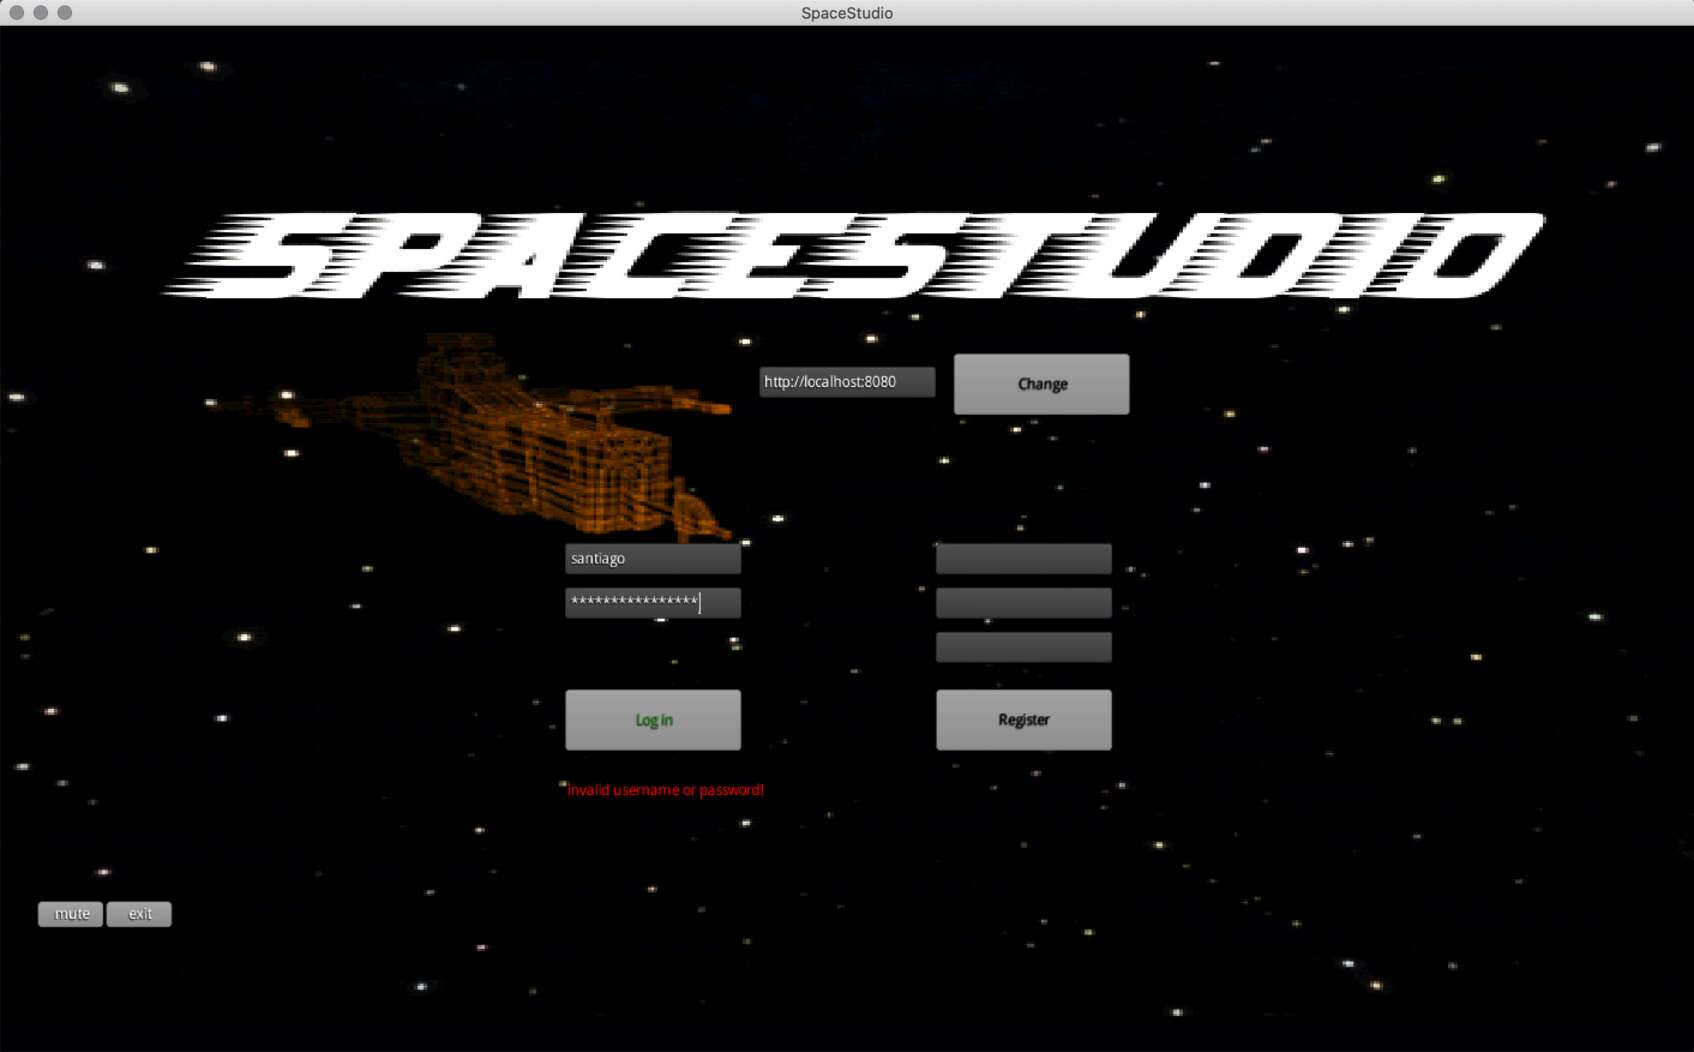
\includegraphics[scale=0.4]{TestProtocolBilder/invalidCredentials.jpg}
\caption{Ungültige Zugangsdaten}
\end{figure}
\newpage
Wenn sich der Benutzer mit gültigen Anmeldeinformationen anmeldet hat, wird der Benutzer zum Menübildschirm weitergeleitet. Falls aber nicht gültige Anmeldedaten verwendet worden sind gibt es eine Fehlermeldung und das Spiel bleibt im Login Screen\\
Eingabe: asdf als Username und fdsa als Passwort.
Diese Anmeldeinformationen gibt es noch nicht, daher gibt es eine Fehlermeldung und es findet keine Weiterleitung statt.\\

\section{Menü Screen}
Tested succesfully by Santiago Rey on 02.08\\\\
Auf dem Menübildschirm sind die Optionen:
\begin{itemize}
\item Continue: Falls ein Spielstand für den Benutzer in der Datenbank gespeichert wurde, wird auch die Option Continue angezeigt. Mit der kann der Benutzer in seinen vorhandenen Spielstand wechseln.\\
Eingabe: Der Spieler drückt auf Continue\\
Ergebnis: Der Spieler kann seinen alten Spielstand fortsetzen.\\
\item New Game: Mit dieser Option kann der Benutzer ein neues Spiel starten.\\
Eingabe: Der Spieler drückt auf New Game.\\
Ergebnis: Der Spieler kommt in den zweiten Menü Screen.\\
\item About: In dieser Option können Informationen zu den Entwicklern gefunden werden.
\item Exit: Mit dieser Option kann der Benutzer das Spiel beenden.
\end{itemize}
\begin{figure}[htp]
\centering
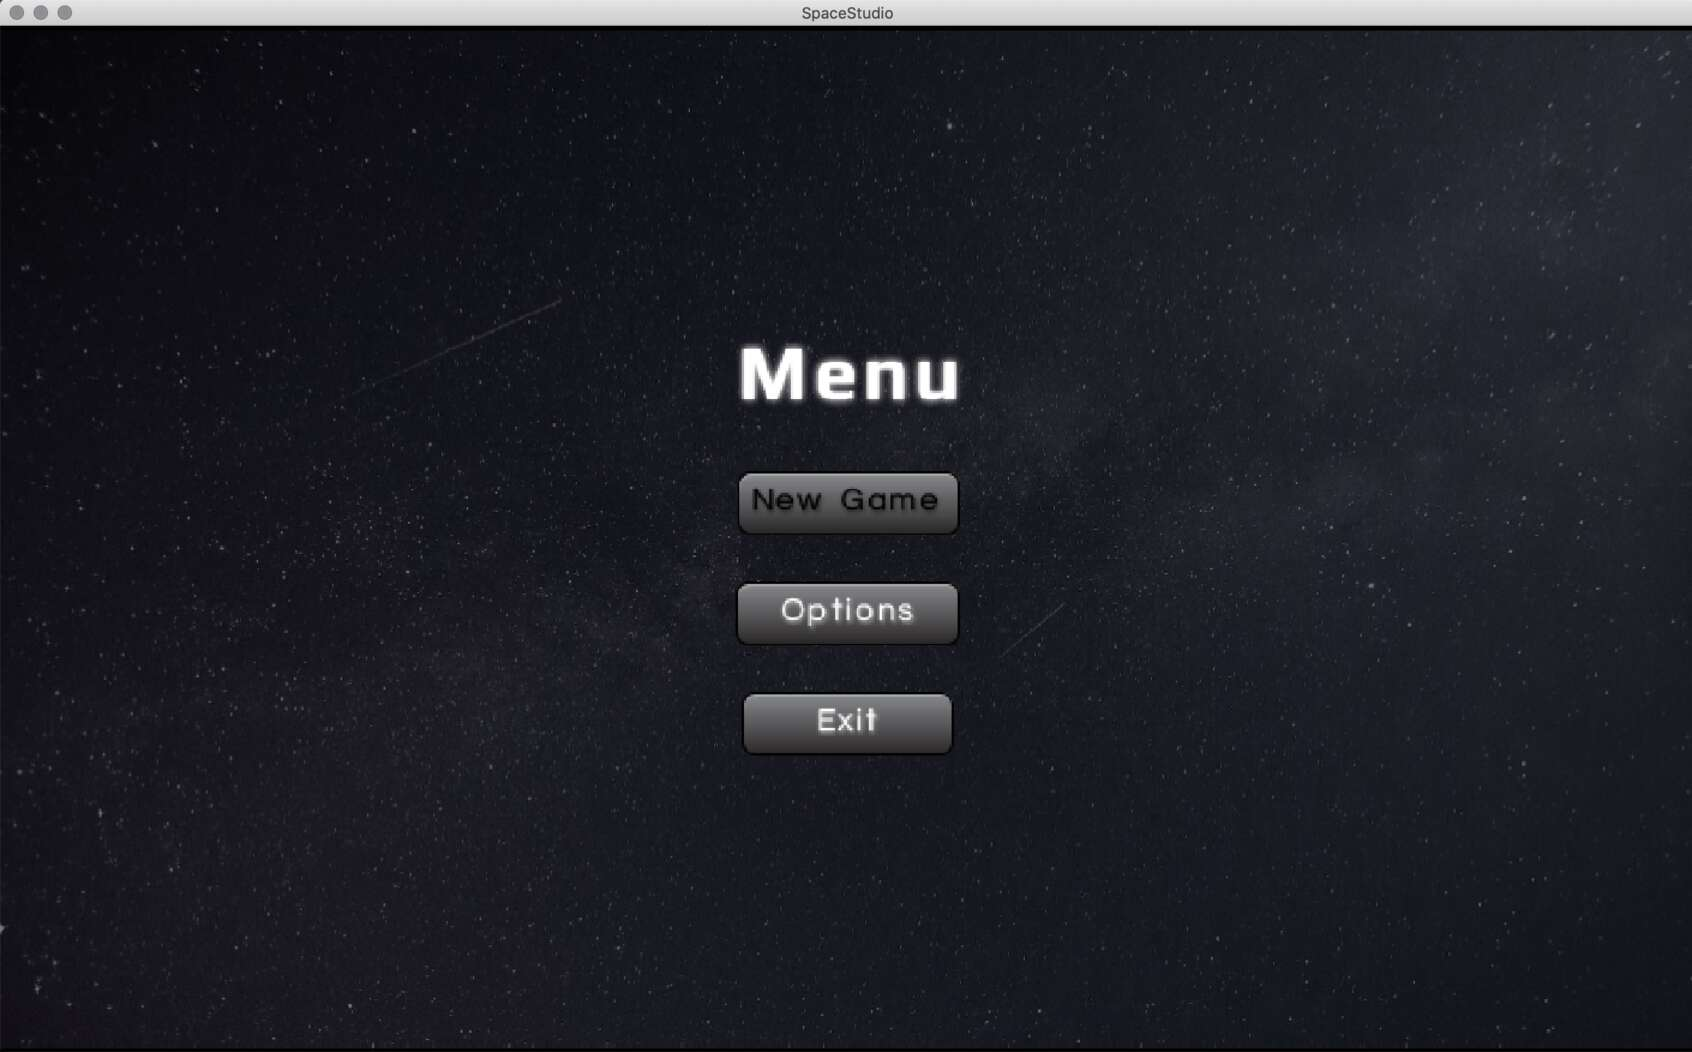
\includegraphics[scale=0.4]{TestProtocolBilder/menuScreen.jpg}
\caption{Menu Spiel}
\end{figure}
\newpage
\section{Spieloptionen}
Tested succesfully by Santiago Rey on 02.08\\\\
Im zweiten Menübildschirm können Sie die Optionen sehen, die der Benutzer spielen muss.
\begin{itemize}
\item Single Player: Mit dieser Option kann der Benutzer als Einzelspieler im Universum spielen.\\
Eingabe: Der Spieler drückt auf die Option Single Player.\\
Ergebnis: Der Spieler gelangt in den Ship-Select-Screen.\\
\item Multiplayer: Diese Option ermöglicht es dem Benutzer, mit einem anderen Spieler im Universum zu spielen und gegeneinander zu kämpfen.\\
Eingabe: Der Spieler drückt auf die Option Multiplayer.\\
Ergebnis: Der Spieler kommt auch in den Ship-Select-Screen\\
\item Back to Menu: Diese Option ermöglicht es Ihnen, zum vorherigen Bildschirm zurückzukehren.
\end{itemize}
\begin{figure}[h]
\centering
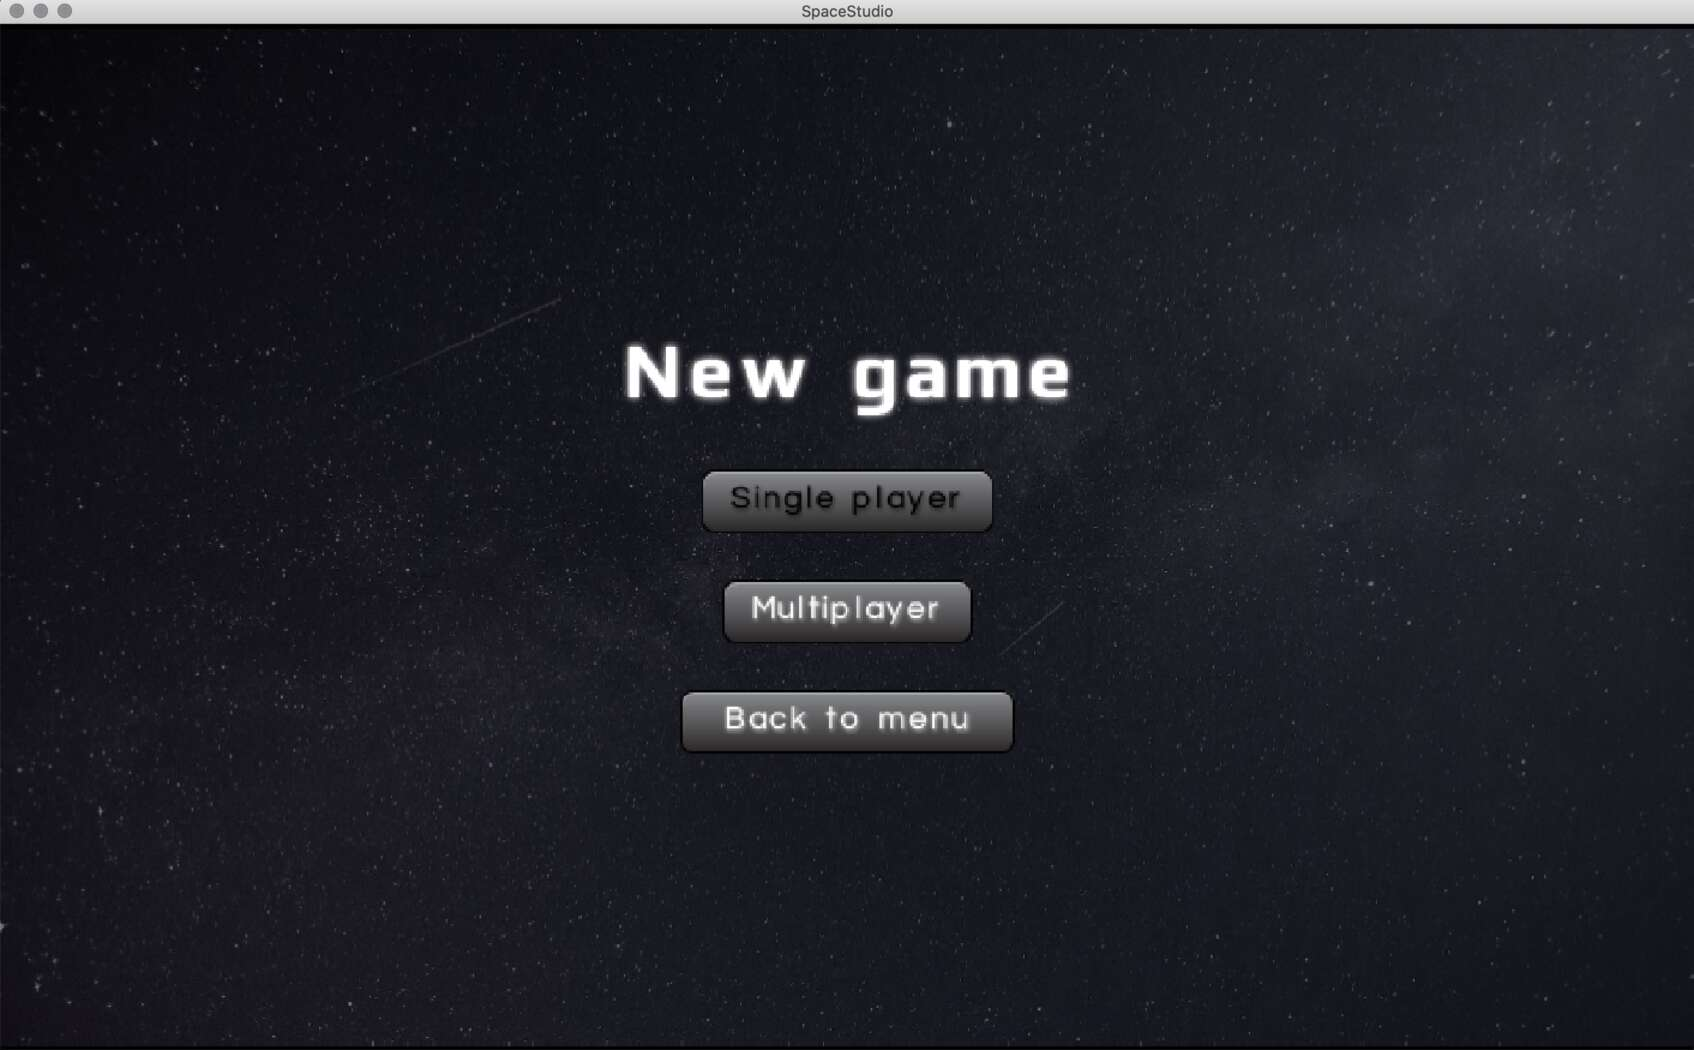
\includegraphics[scale=0.4]{TestProtocolBilder/menuScreenTwo.jpg}
\caption{Spieloptionen}
\end{figure}
\newpage
\section{Testfall Single Player}
Tested succesfully by Santiago Rey on 02.08\\\\
Auf diesem Bildschirm wurde jede Schaltfläche getestet, beginnend mit der Taste Single Player.\\
\begin{figure}[h]
\centering
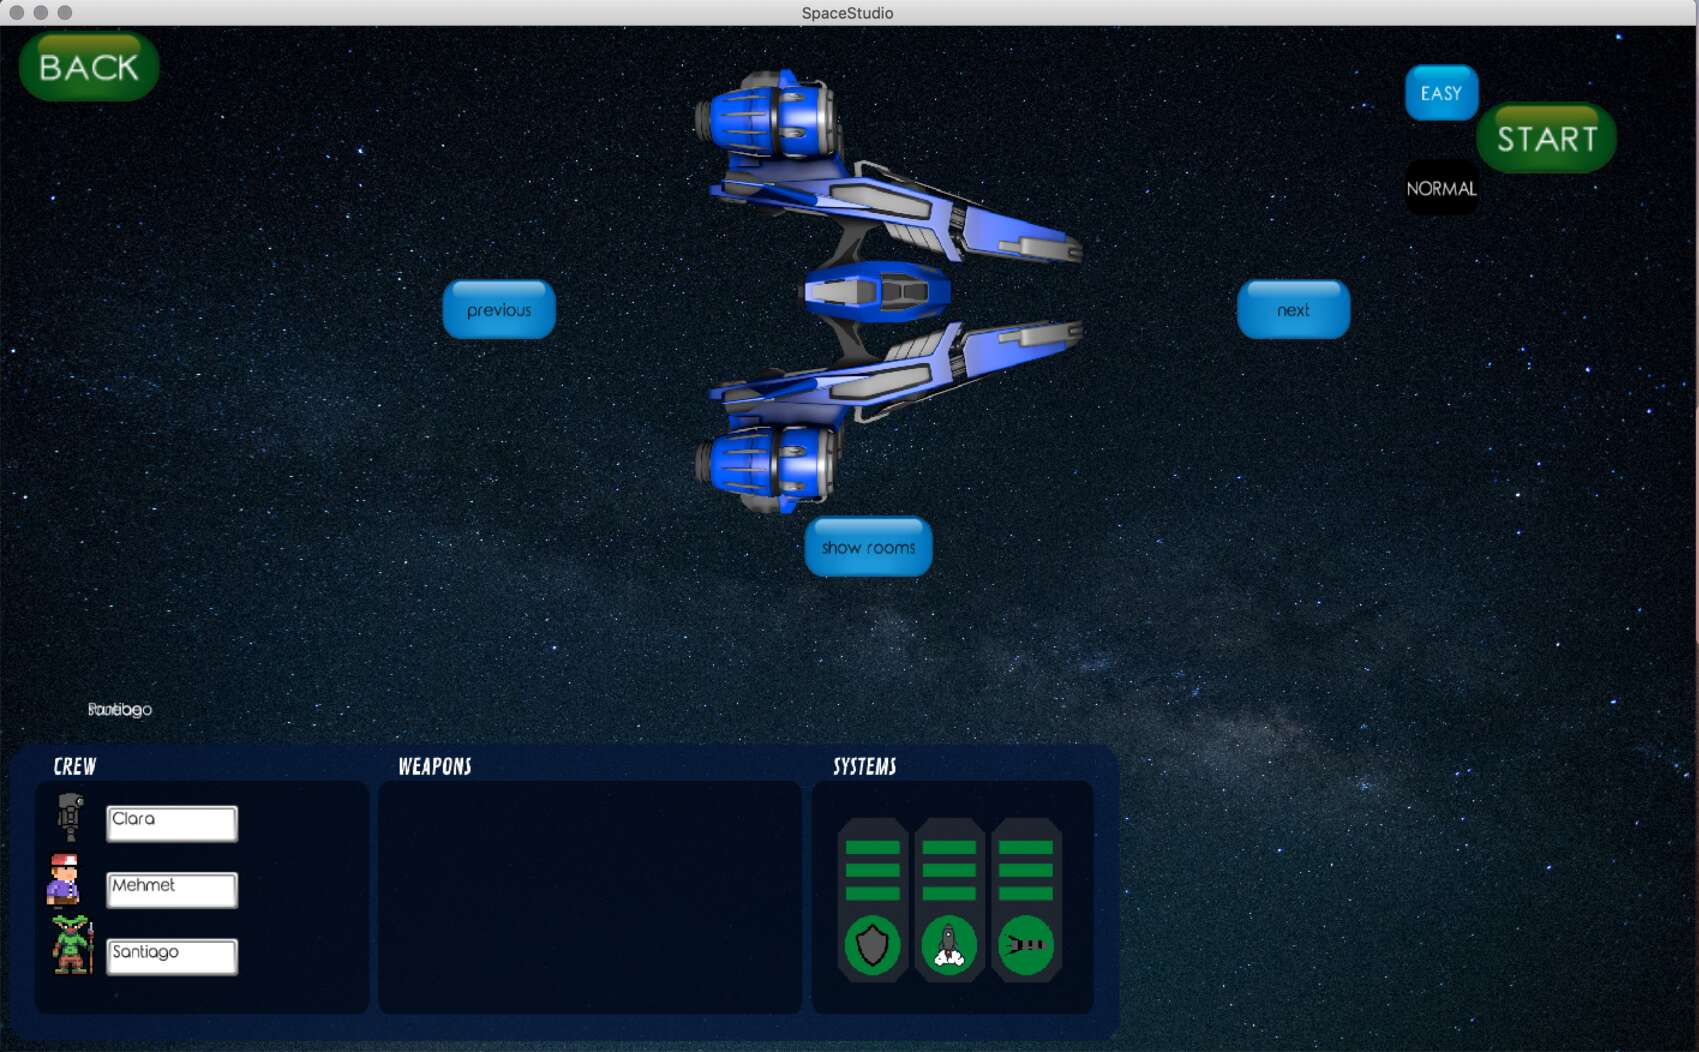
\includegraphics[scale=0.4]{TestProtocolBilder/selecShipScreen.jpg}
\caption{Select Ship screen}
\end{figure}
\newpage
\subsection{Sektionen anzeigen Test}
Tested succesfully by Santiago Rey on 02.08\\\\
Mit dem Button "show rooms" wurde getestet, ob die Sektionen des Raumschiffes sichtbar sind. Wenn Sie erneut drücken, verschwinden die Abschnitte\\
\begin{figure}
\centering
\includegraphics[scale=0.4]{TestProtocolBilder/shipRooms.jpg}
\caption{Sektionen des Raumschiffs}
\end{figure}

\newpage

\subsection{Andere Raumschiffe}
Tested succesfully by Santiago Rey on 02.08\\\\
Mit der nächsten Schaltfläche kann der Benutzer die möglichen Schiffe für das Spiel sehen.\\
Eingabe: Spieler drückt auf next und previous.\\
Ergebnis: Spieler sieht alle anderen verfügbaren Raumschiffe.
\begin{figure}
\centering
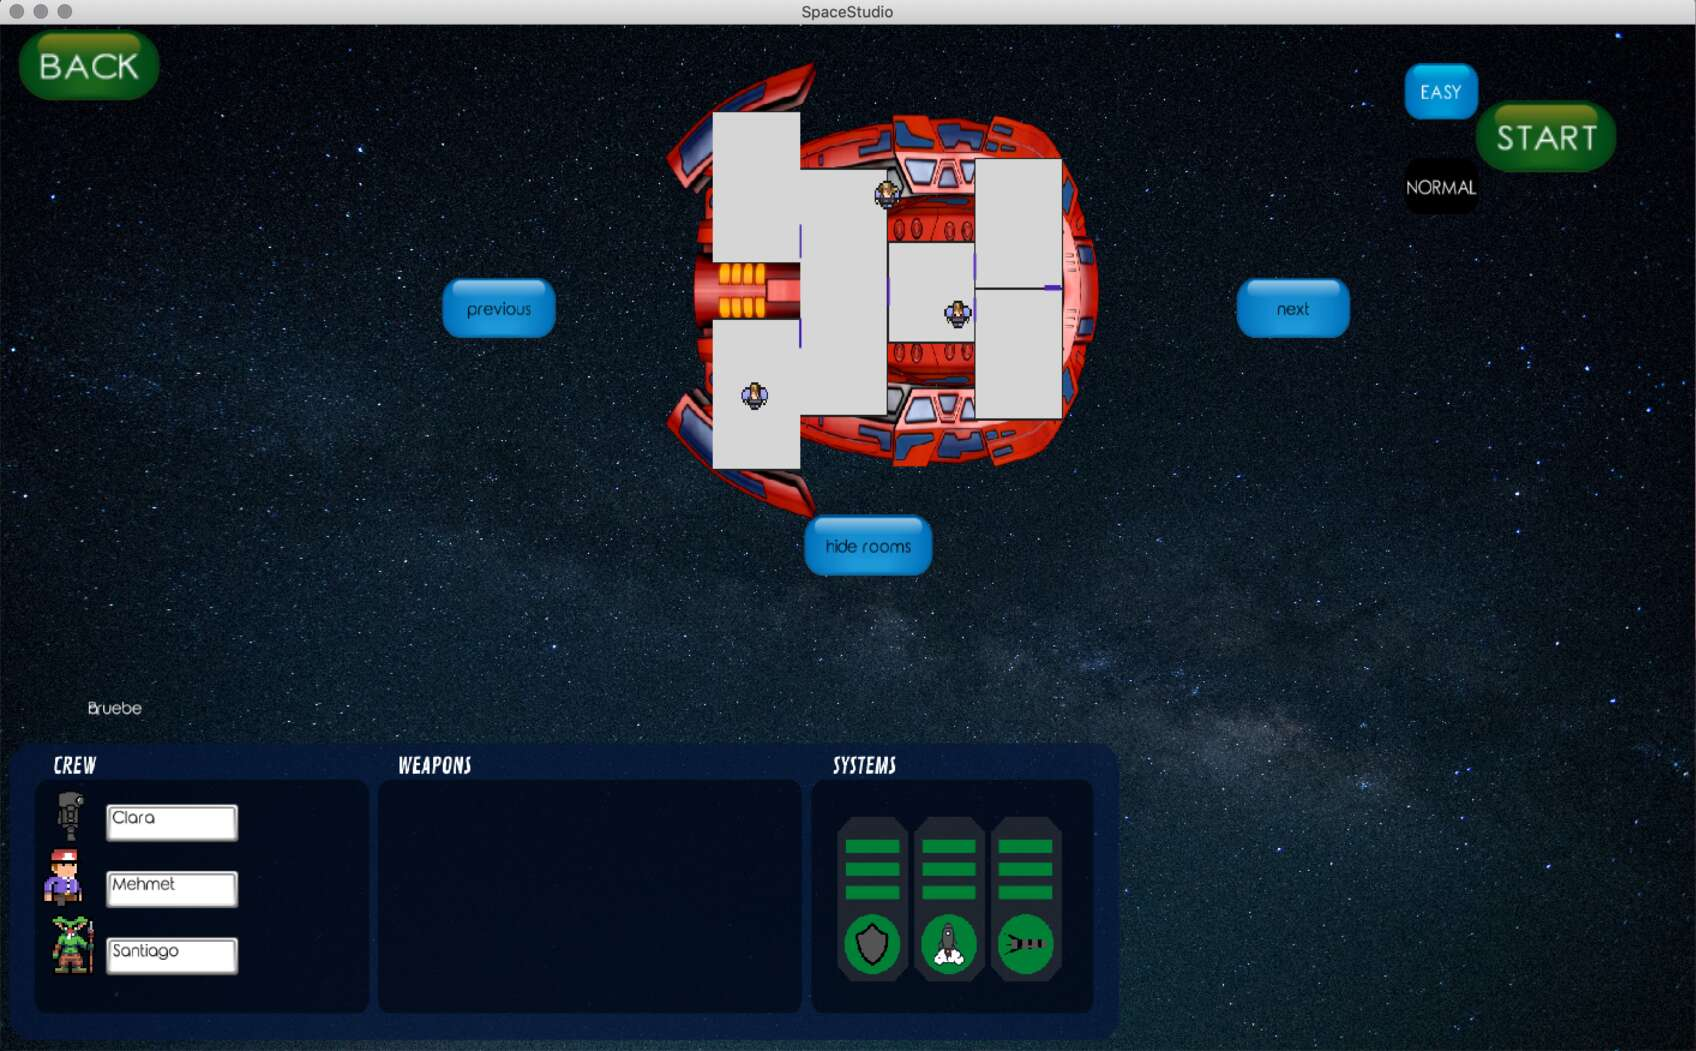
\includegraphics[scale=0.4]{TestProtocolBilder/next.jpg}
\caption{Andere mögliche Raumschiffe}
\end{figure}

\newpage
\subsection{Universum Schwierigkeit}
Tested succesfully by Santiago Rey on 02.08\\\\
Diese Testschaltfläche ermöglicht die Schaffung eines größeren Universums, in dem es mehr Planeten mit unterschiedlichen Eigenschaften gibt.\\
Eingabe: Der Spieler sucht einen der Schwierigkeiten und startet das Spiel.\\
Ergebnis: Das Spiel startet in der ausgewählten Schwierigkeit.
\begin{figure}
\centering
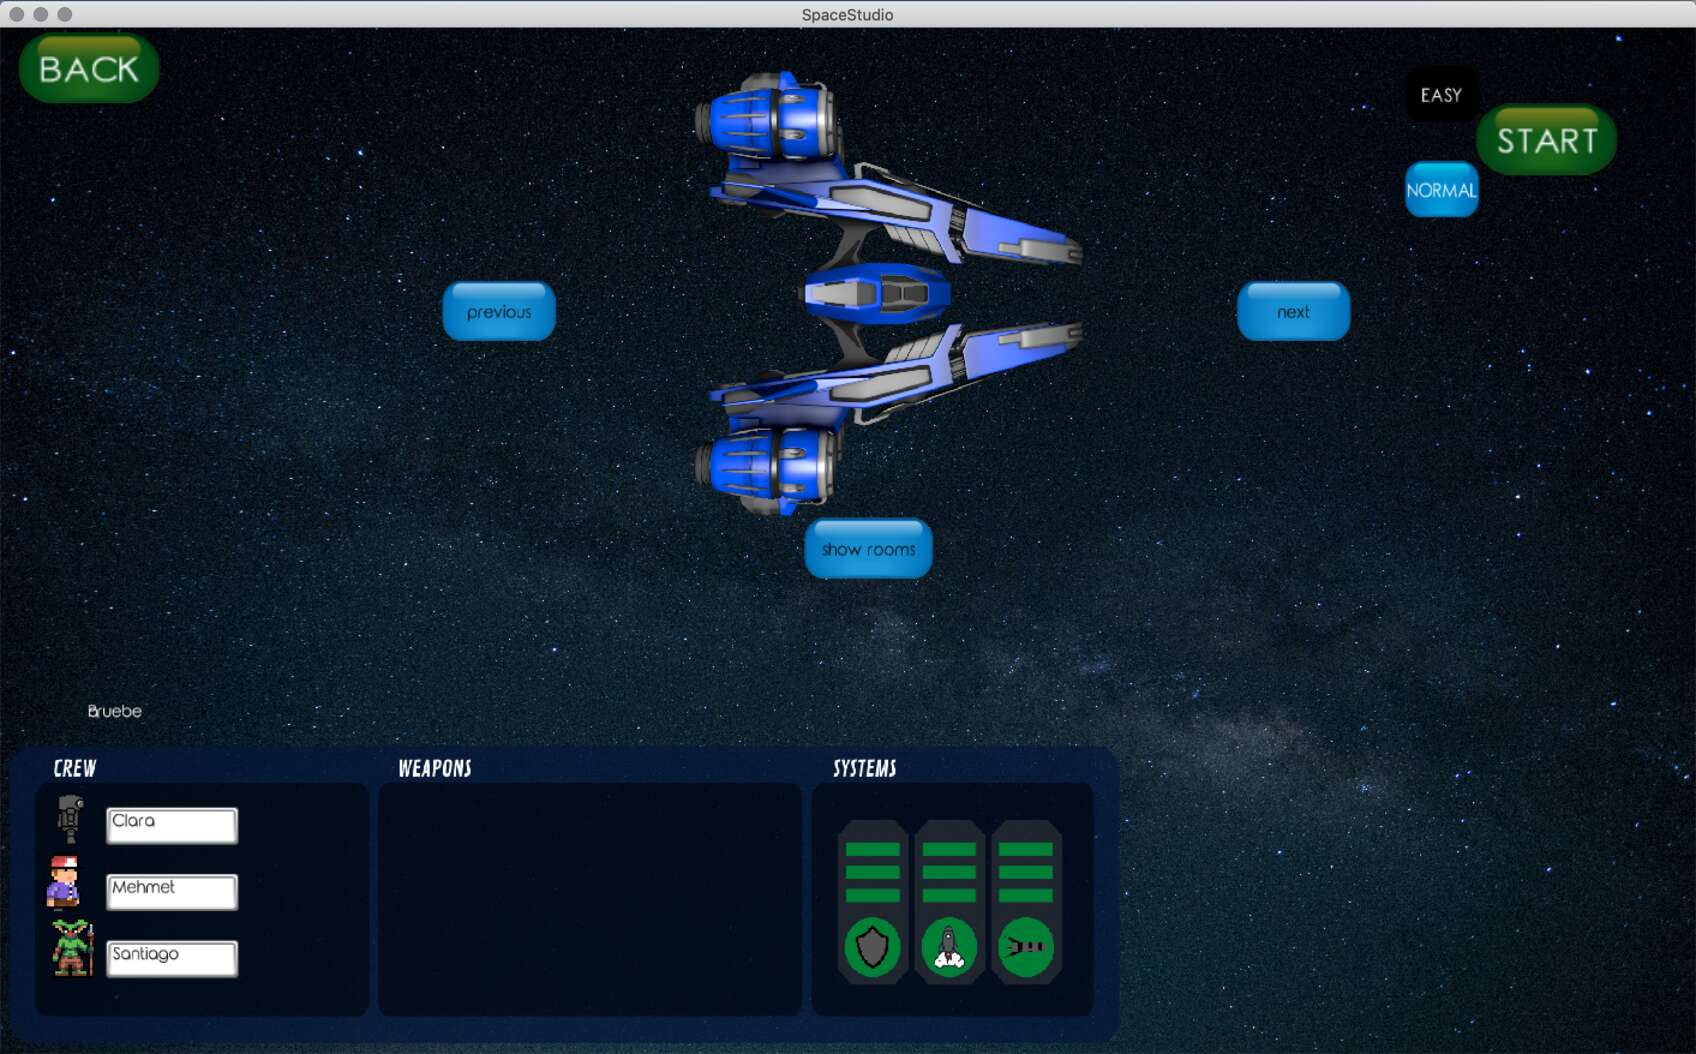
\includegraphics[scale=0.4]{TestProtocolBilder/universeButon.jpg}
\caption{Leichte und normale Schwierigkeit}
\end{figure}

\newpage
Das Universum mit einer komplexeren Schwierigkeit wird korrekt erstellt.\\

\begin{figure}[t]
\centering
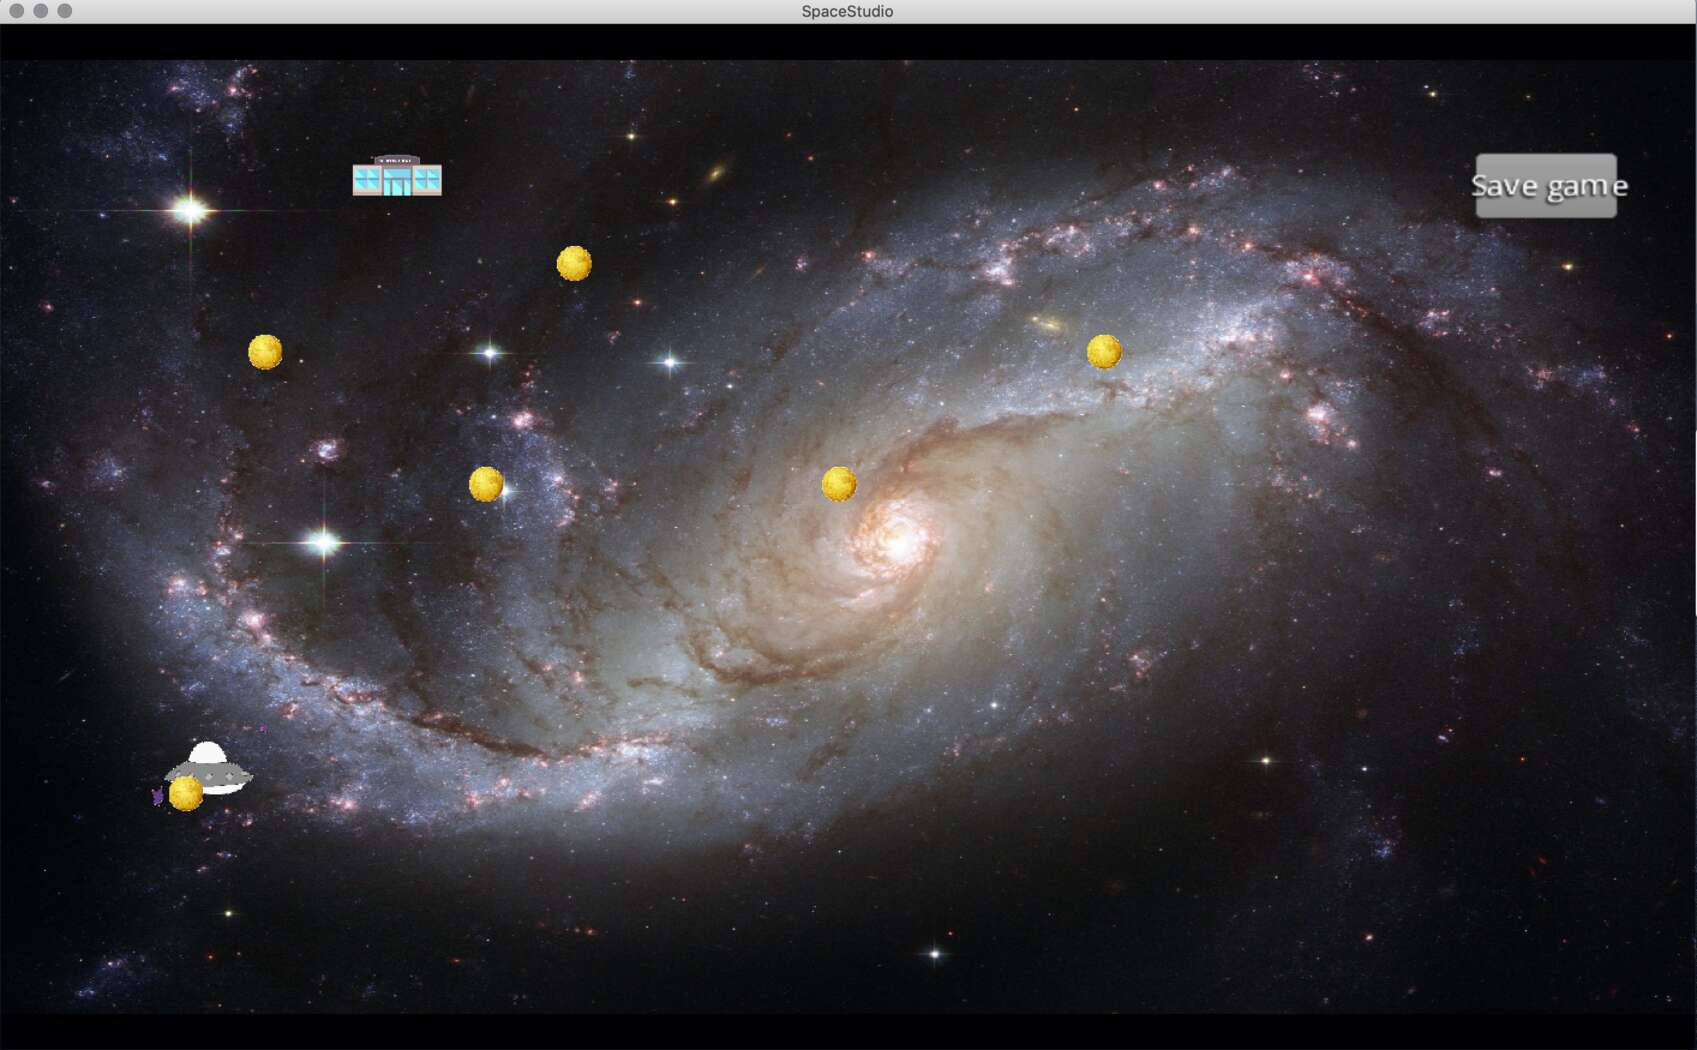
\includegraphics[scale=0.4]{TestProtocolBilder/universeHard.jpg}
\caption{Universum normal Schwierigkeit}
\end{figure}

Die Schaltfläche, die das Beenden des Universums erleichtert, wurde ebenfalls getestet.\\

\begin{figure}[t]
\centering
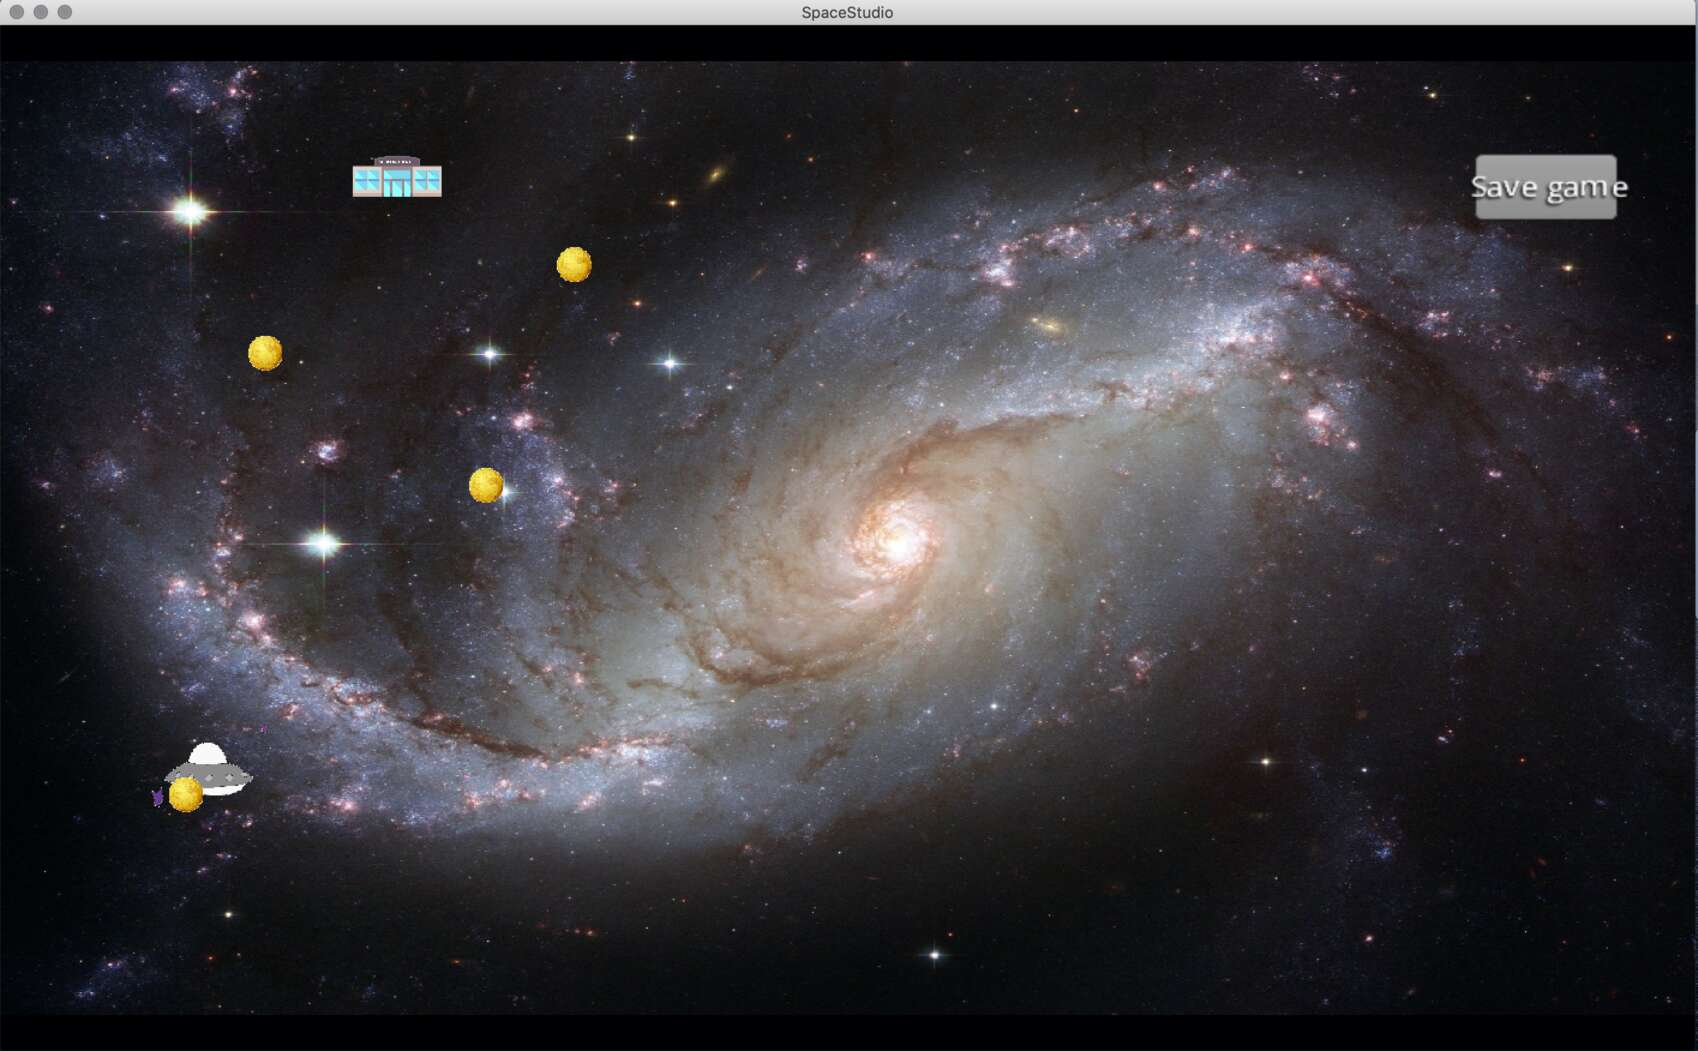
\includegraphics[scale=0.4]{TestProtocolBilder/universeEase.jpg}
\caption{Universum im leichten Schwierigkeitsmodus}
\end{figure}

\newpage
\subsection{Karte}
Tested succesfully by Santiago Rey on 02.08\\\\
Hier wurde jeder Planet und jede Station getestet, die Schaltflächen sind der Zugang zum Ereignis-Bildschirm.\\
\begin{figure}
\centering
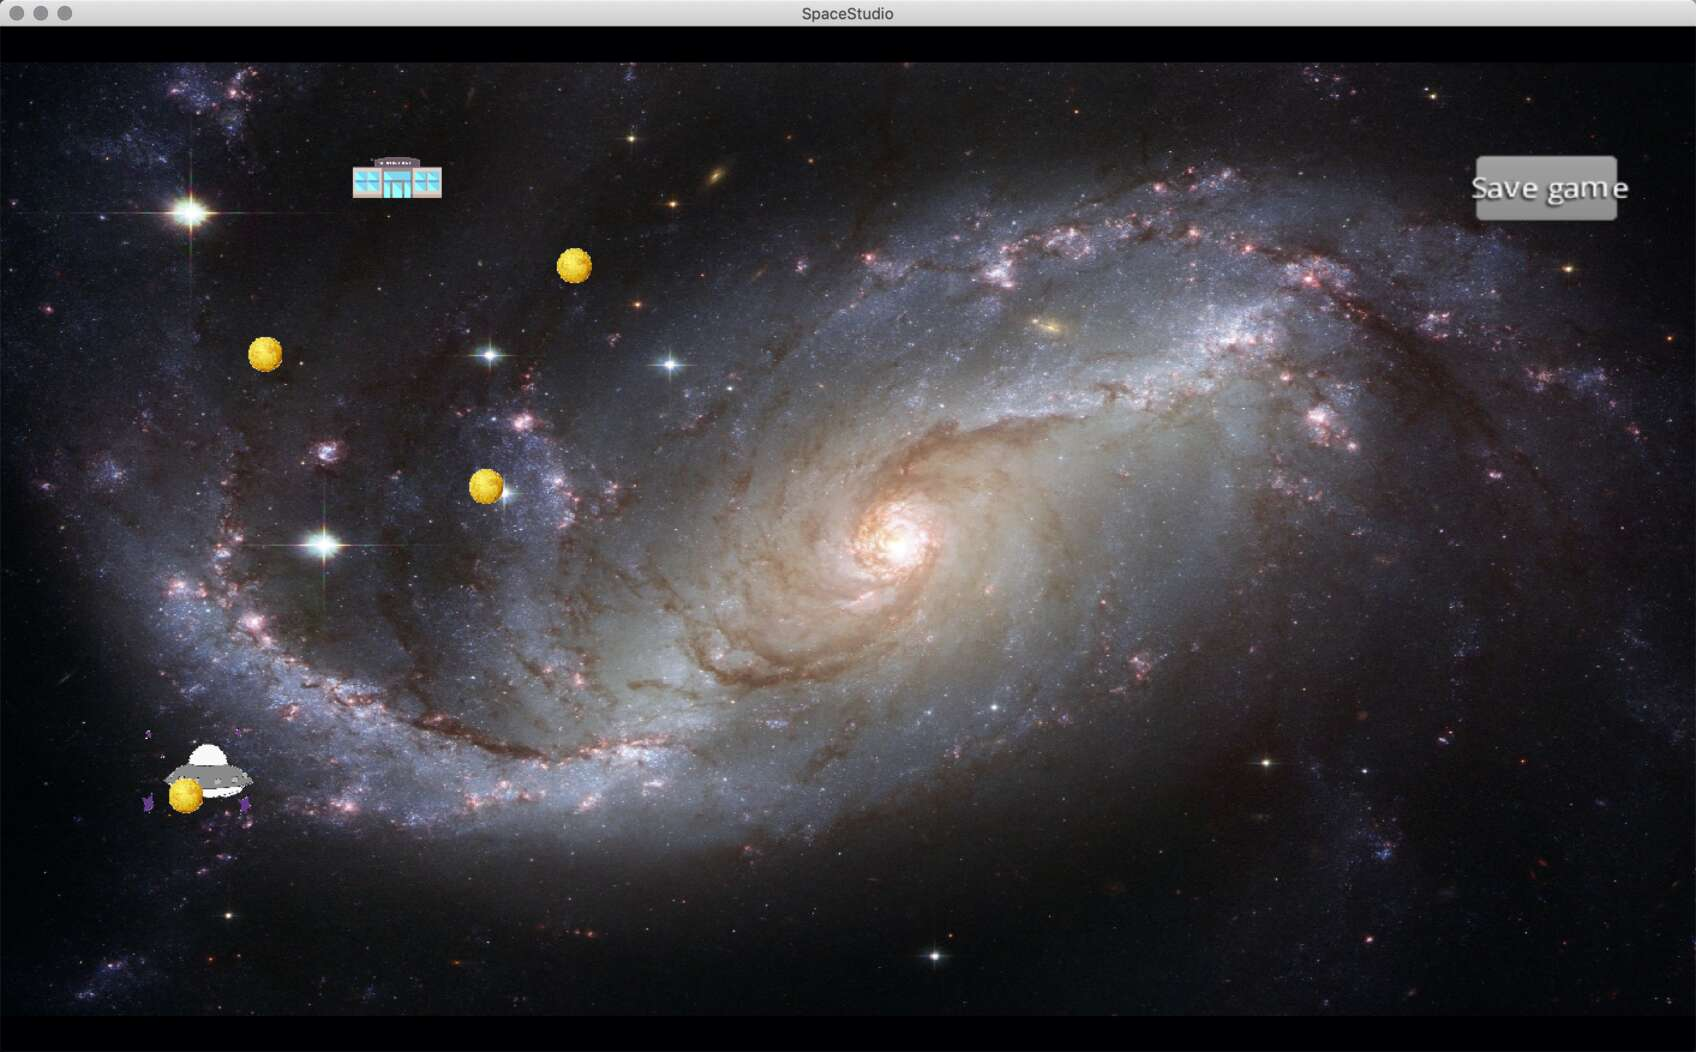
\includegraphics[scale=0.4]{TestProtocolBilder/map.jpg}
\caption{Game Map}
\end{figure}
\newpage
\section{Ereignisse}
Tested succesfully by Santiago Rey on 02.08\\\\
Nach dem Drücken eines Planeten wird ein Popup-Menü angezeigt und die Springfunktion getestet. Nach Auswahl der Springfunktion sieht der Benutzer auf dem Bildschirm eine Fahrzeit von 4 Sekunden.\\
Eingabe: Der Spieler drückt auf einen Planeten.\\
Ergebnis: Der Spieler gelangt zu dem ausgewählten Planeten und kann hat mehrere Optionen wie z.B. Fight.
\begin{figure}[htp]
\centering
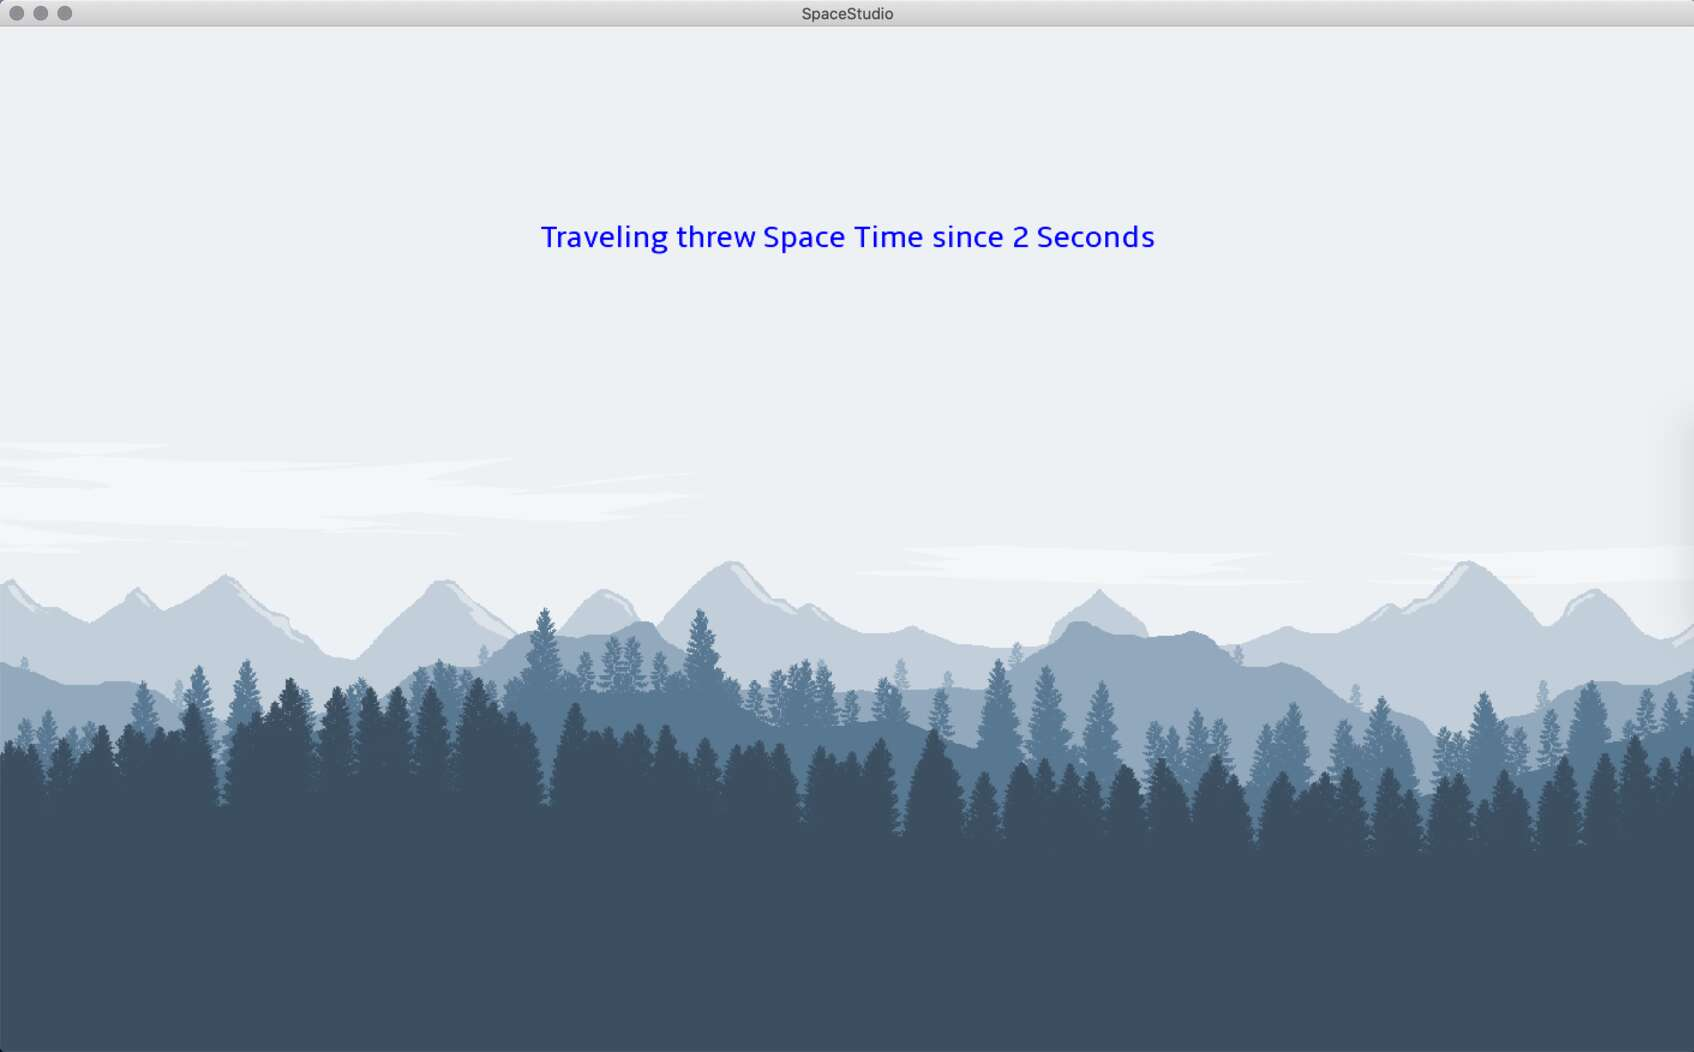
\includegraphics[scale=0.4]{TestProtocolBilder/traveling.jpg}
\caption{Reise Screen}
\end{figure}
\clearpage
Der Button flee, dann man kann wieder auf die Map Screen springen.\\
Eingabe: Der Spieler drückt auf den Button flee.\\
Ergebnis: Der Spieler bleibt auf der Kartenansicht und kann auf eine andere Station/Planet fliegen.\\
\newpage
\subsection{Fliehen}
\begin{figure}[htp]
\centering
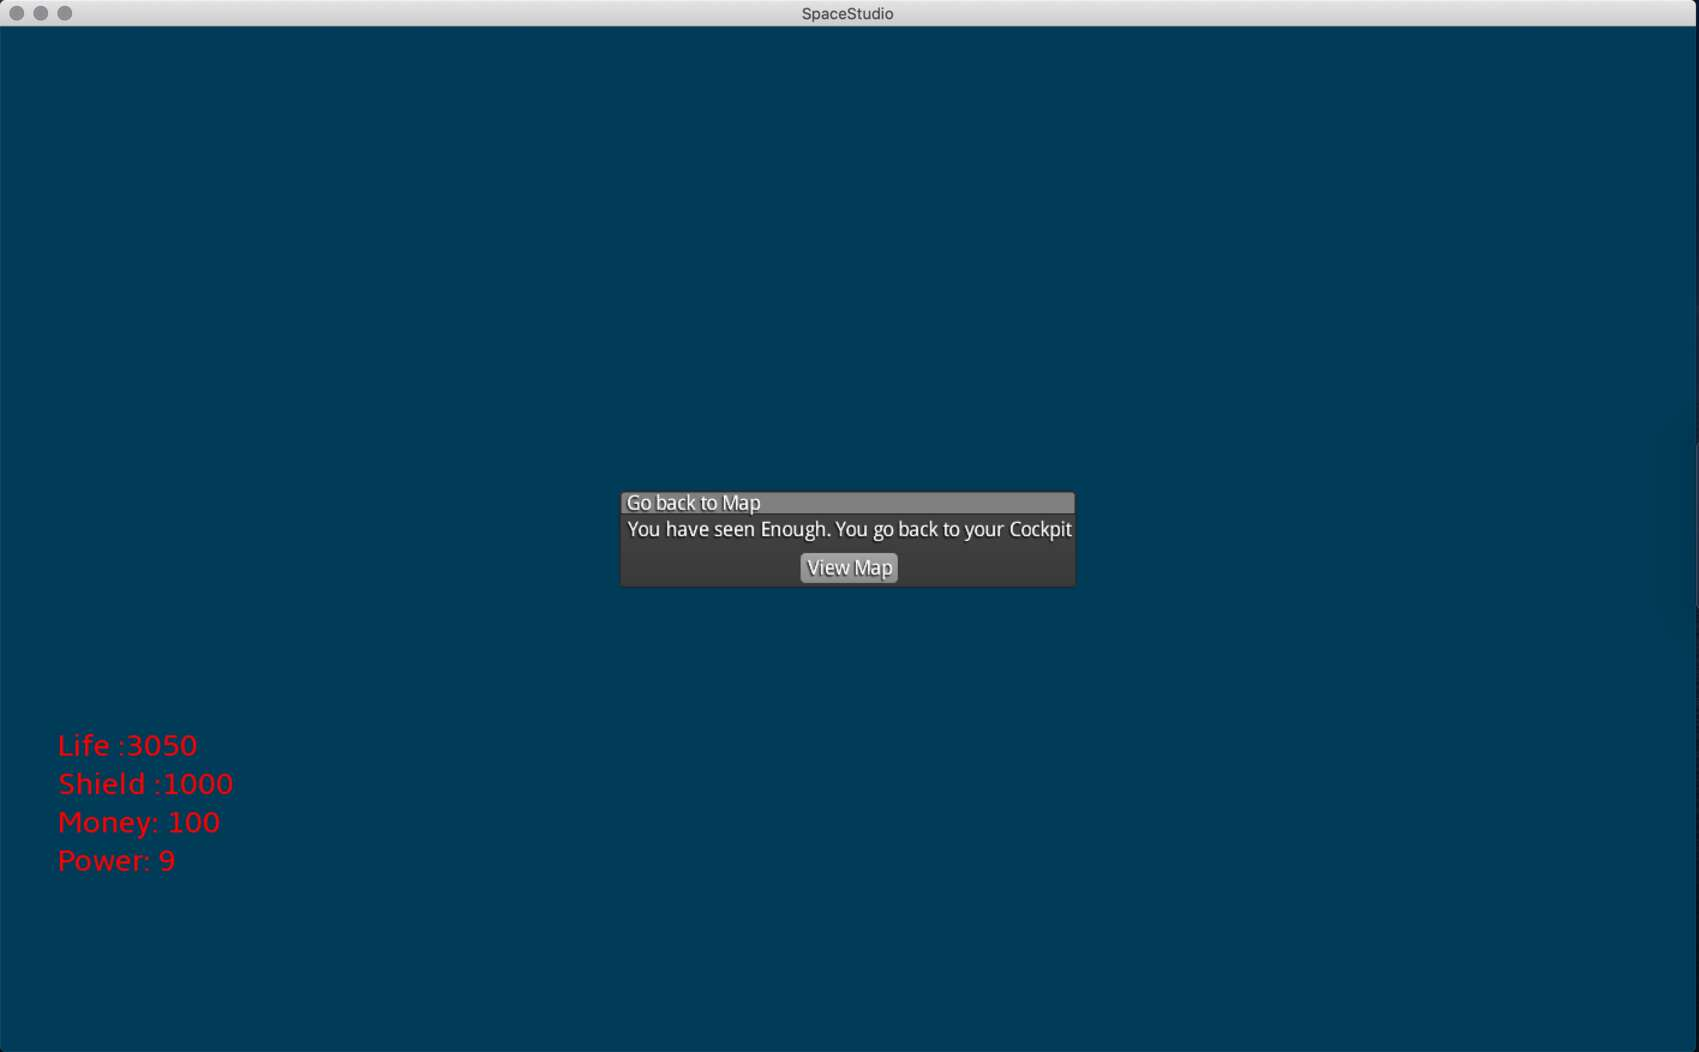
\includegraphics[scale=0.4]{TestProtocolBilder/flee.jpg}
\caption{Fliehen Screen Button}
\end{figure}
\newpage
Es wurde getestet, dass nach dem Reisebildschirm der erste Teil der Ereignisse angezeigt wird.\\
\begin{figure}[htp]
\centering
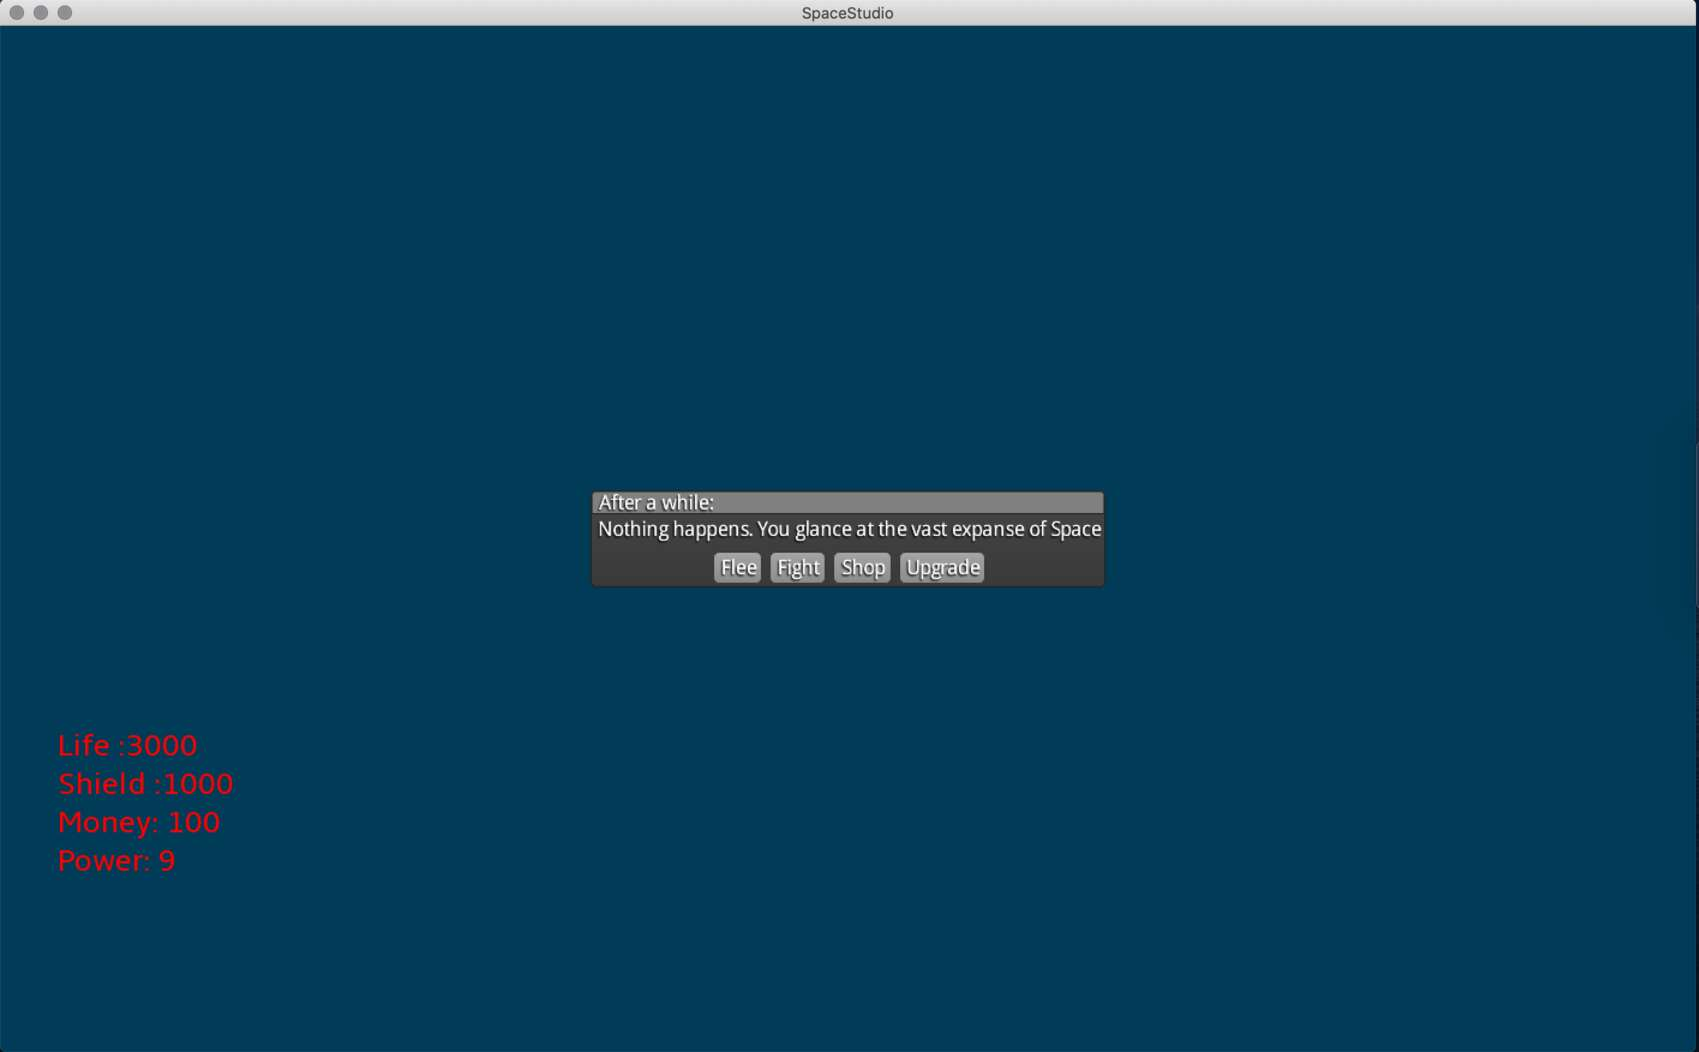
\includegraphics[scale=0.4]{TestProtocolBilder/InitialGeeinisse.jpg}
\caption{Erste Ereignisse}
\end{figure}
\clearpage
Dieser Bildschirm war für die Einführung des Benutzers in die Ereignisse gedacht.\\
Andere Arten von Ereignissen wurden getestet, insgesamt gibt es fünf verschiedene Arten von Ereignissen pro Universum.
\begin{figure}[htp]
\centering
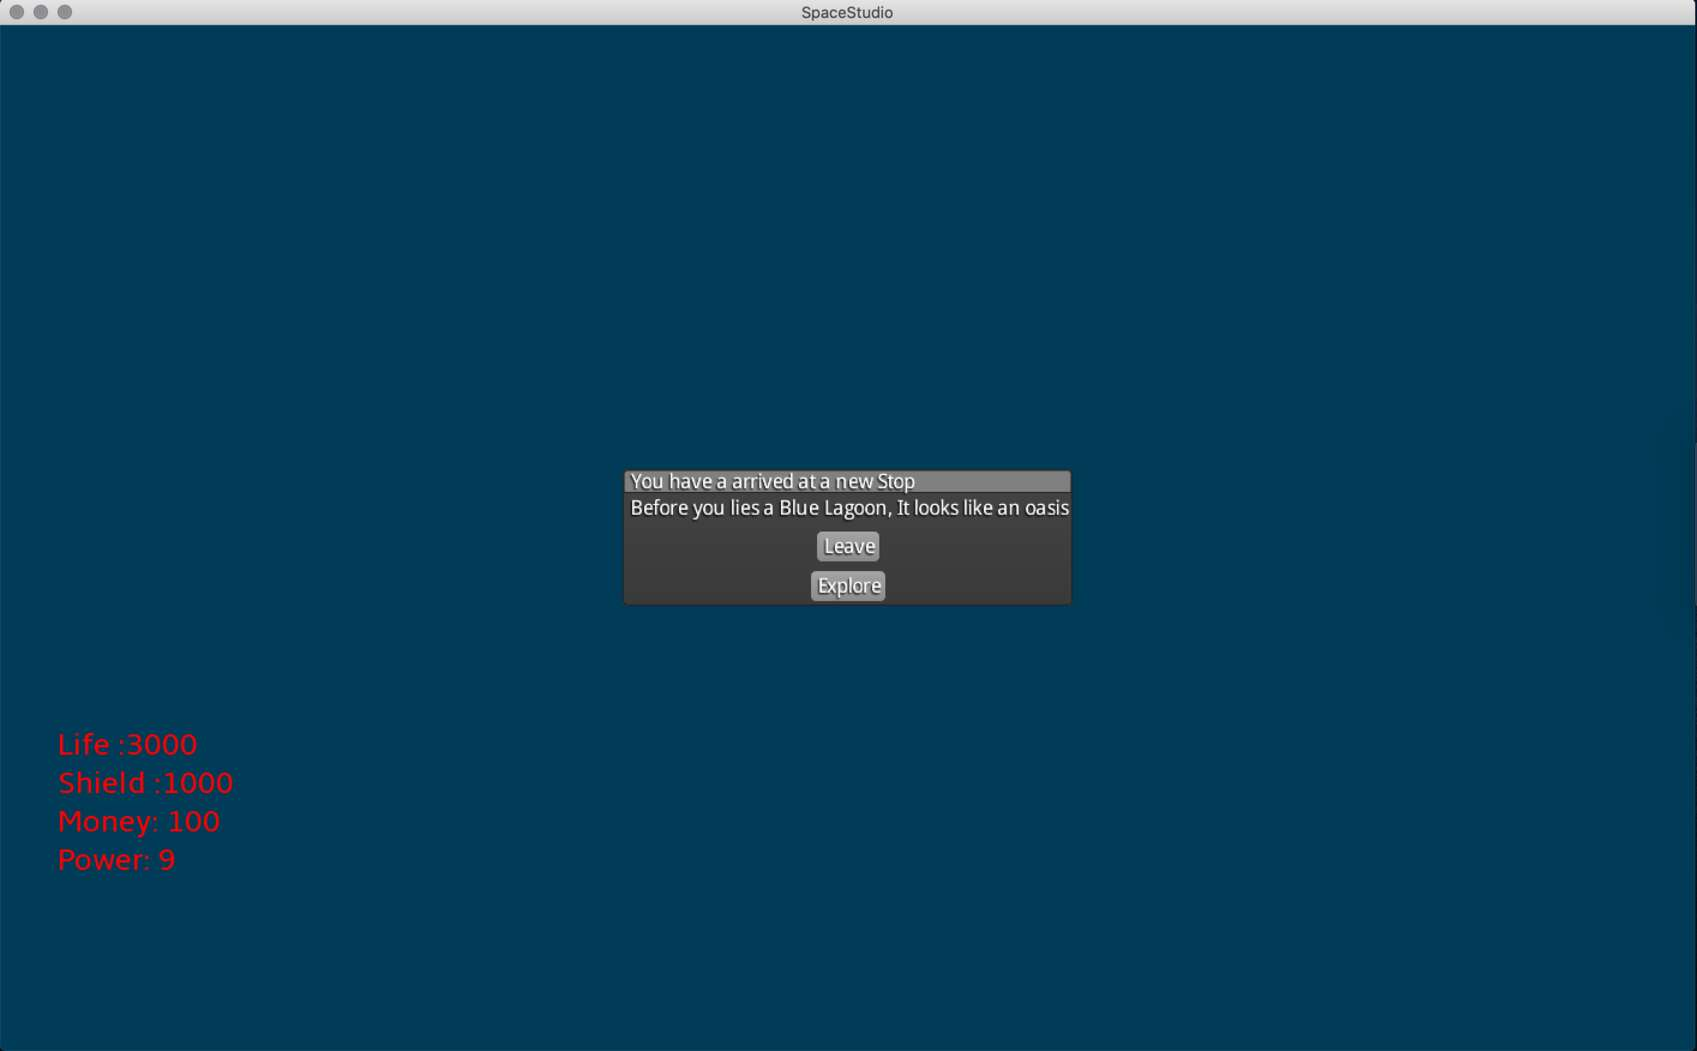
\includegraphics[scale=0.4]{TestProtocolBilder/otherEreignisse.jpg}
\caption{Anderer Typ von Ereignissen}
\end{figure}
Sobald Sie den Einkaufsteil des Spiels betreten, können Sie die in diesem Teil verfügbaren Dinge kaufen.\\
Eingabe: Der Spieler drückt auf die Station Shop.\\
Ergebnis: Der Spieler gelangt in den Shop-Screen und gelangt in den Shop und kann dort Waffen, Crewmember, Energie und vieles mehr kaufen.
\begin{figure}[htp]
\centering
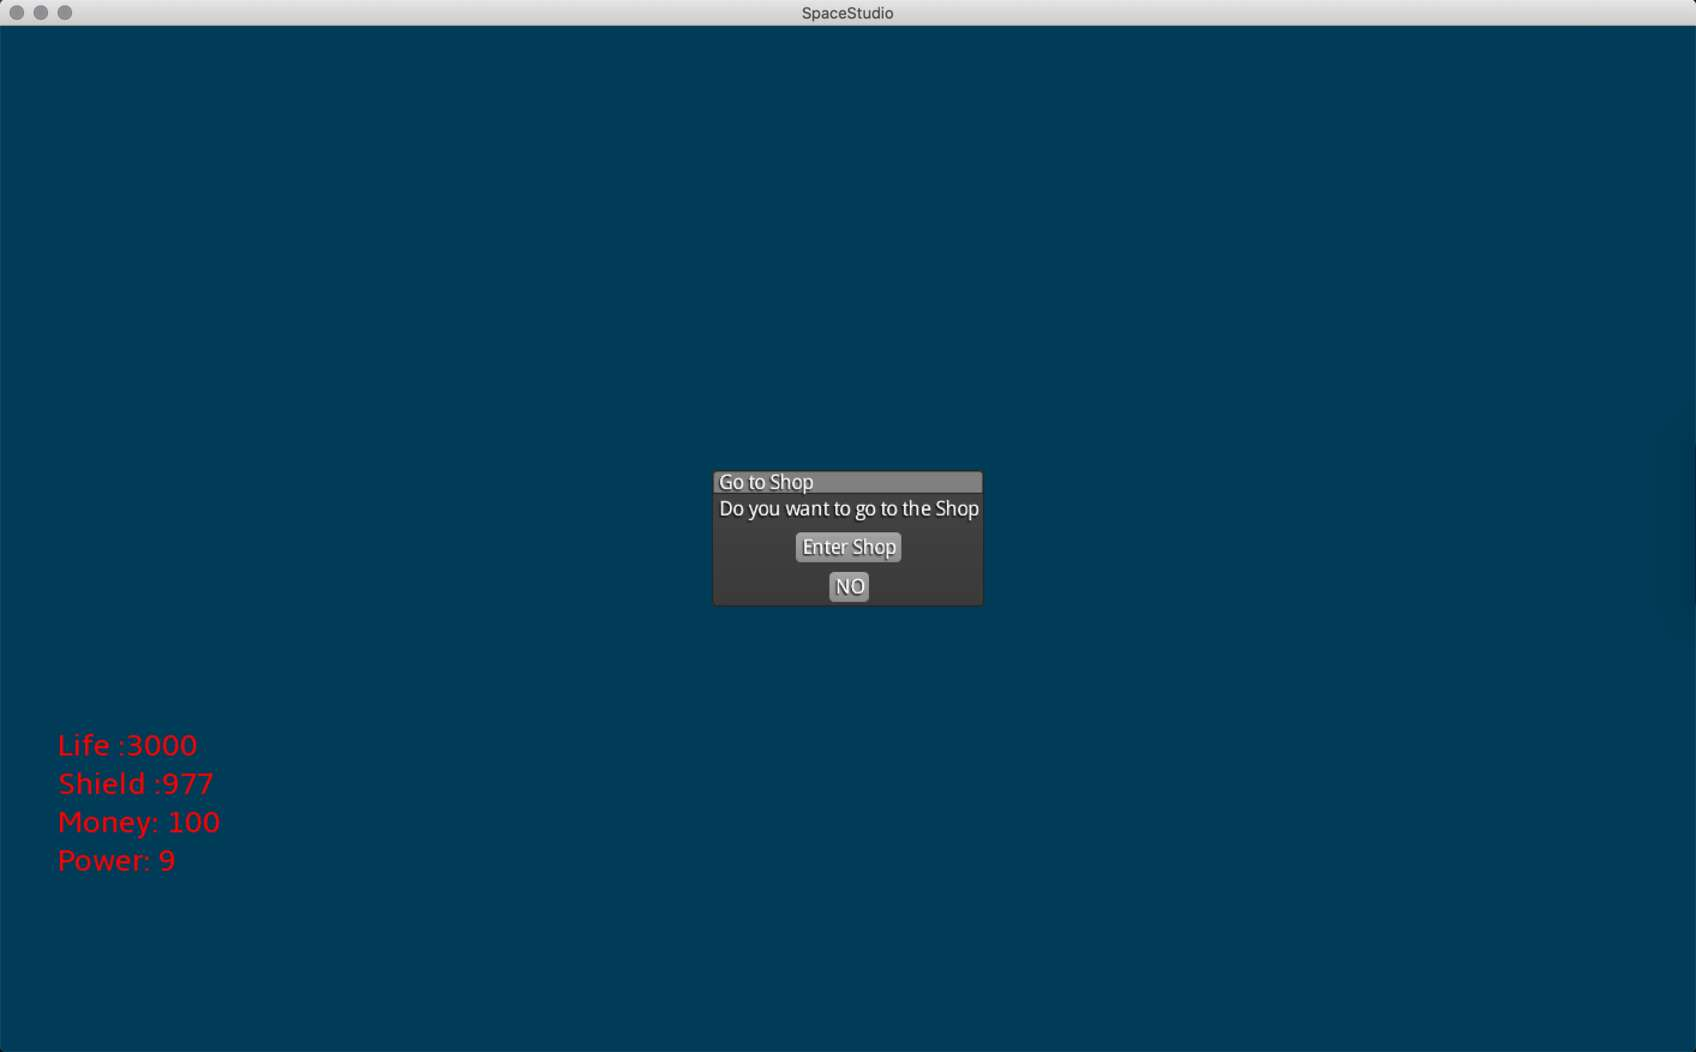
\includegraphics[scale=0.4]{TestProtocolBilder/shopPlanetJump.jpg}
\caption{Springen zur Shop-Station}
\end{figure}
\newpage
\section{Shop Screen}
Tested succesfully by Santiago Rey on 02.08\\\\
Wenn der Benutzer den Shop-Bildschirm betritt, kann er den Kaufen-Button und die verfügbaren Ressourcen sehen.
\begin{figure}[h]
\centering
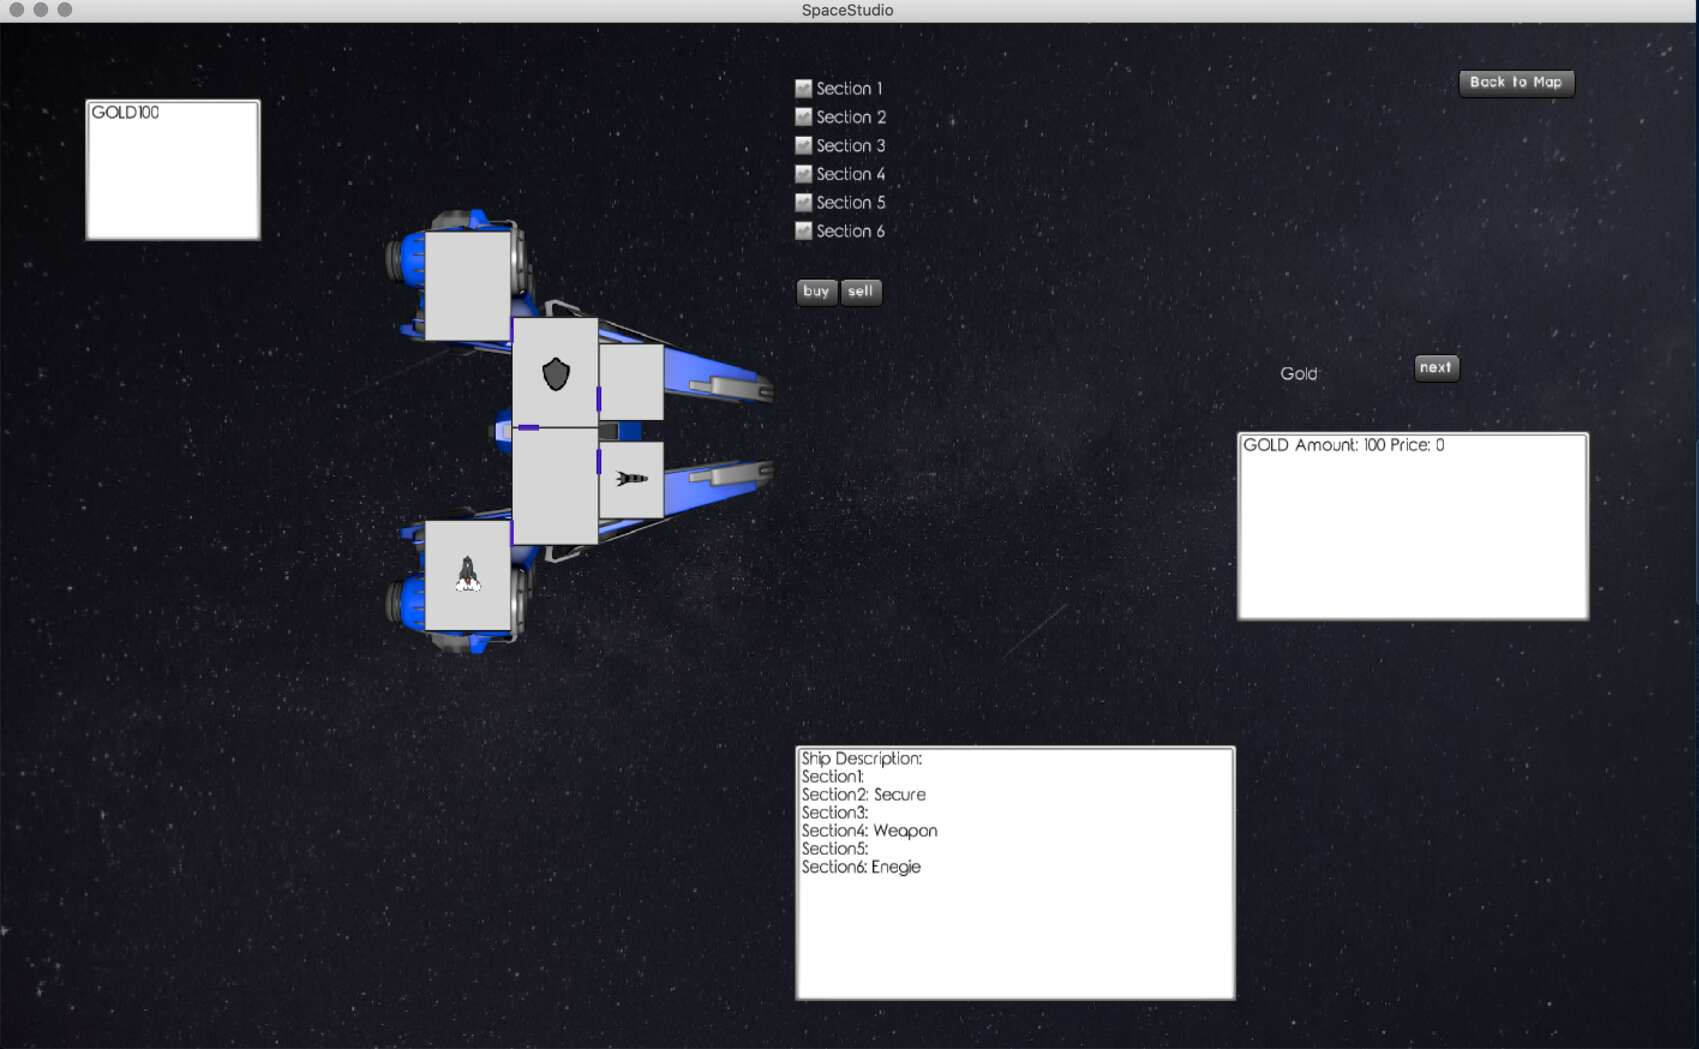
\includegraphics[scale=0.4]{TestProtocolBilder/shopScreen.jpg}
\caption{shop Screen}
\end{figure}

\subsection{Kaufen}
Als nächstes wurde der Kauf jedes Objekts sowie das Ergebnis des verbleibenden Geldes des Spielers getestet.\\
Eingabe: Der Spieler kauft ein Objekt.
Ergebnis: Das Gold wird reduziert und der Spieler bekommt das Objekt.
\subsubsection{Gold kaufen}
Dies ist das Ergebnis nach dem Kauf von Gold, was sich direkt auf das Geld des Benutzers auswirkt.
\begin{figure}[htp]
\centering
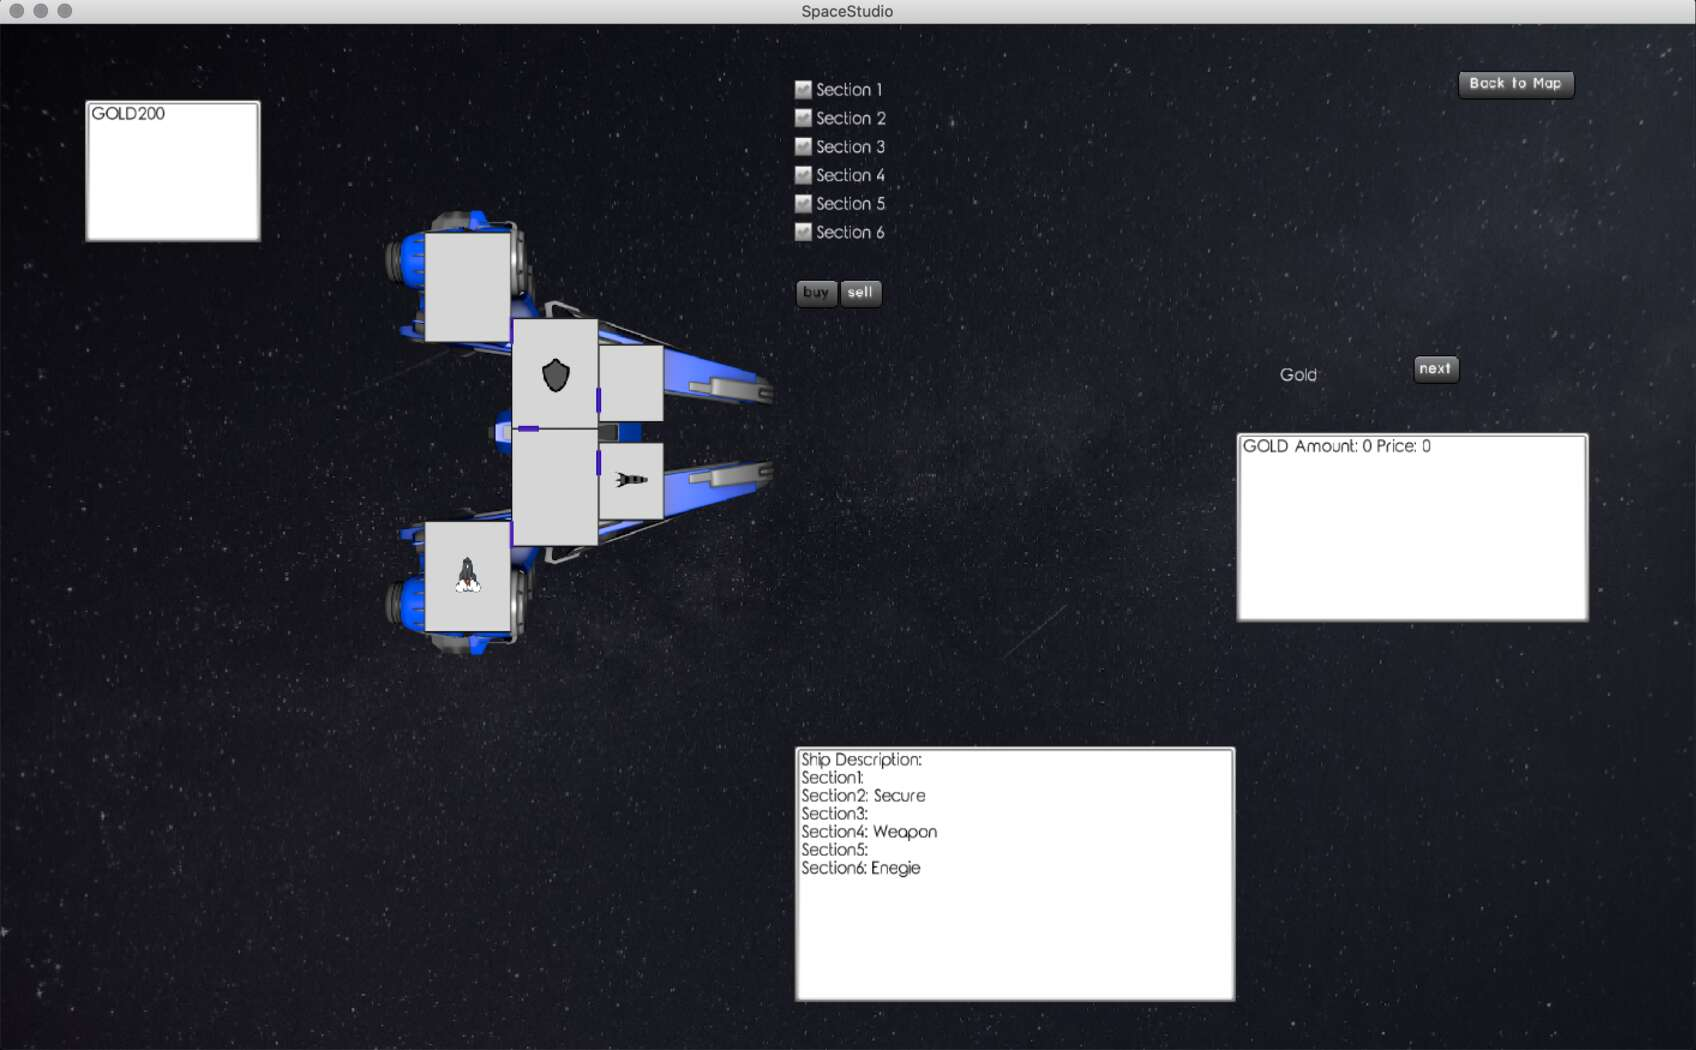
\includegraphics[scale=0.4]{TestProtocolBilder/goldgekauft.jpg}
\caption{Anderer Typ von Ereignissen}
\end{figure}
\newpage
\subsubsection{Energie kaufen}
Dies ist das Ergebnis nach dem Kauf von Energie. Dieser Kauf wirkt sich auf das Raumschiff aus und es ist nur möglich, die Reduzierung von Gold auf dem Raumschiff zu sehen.\\
Eingabe: Der Spieler kauft Energie.\\
Ergebnis: Der Spieler bekommt Energie und kann diese den vorhandenen Systemen zuteilen.\\
\begin{figure}[htp]
\centering
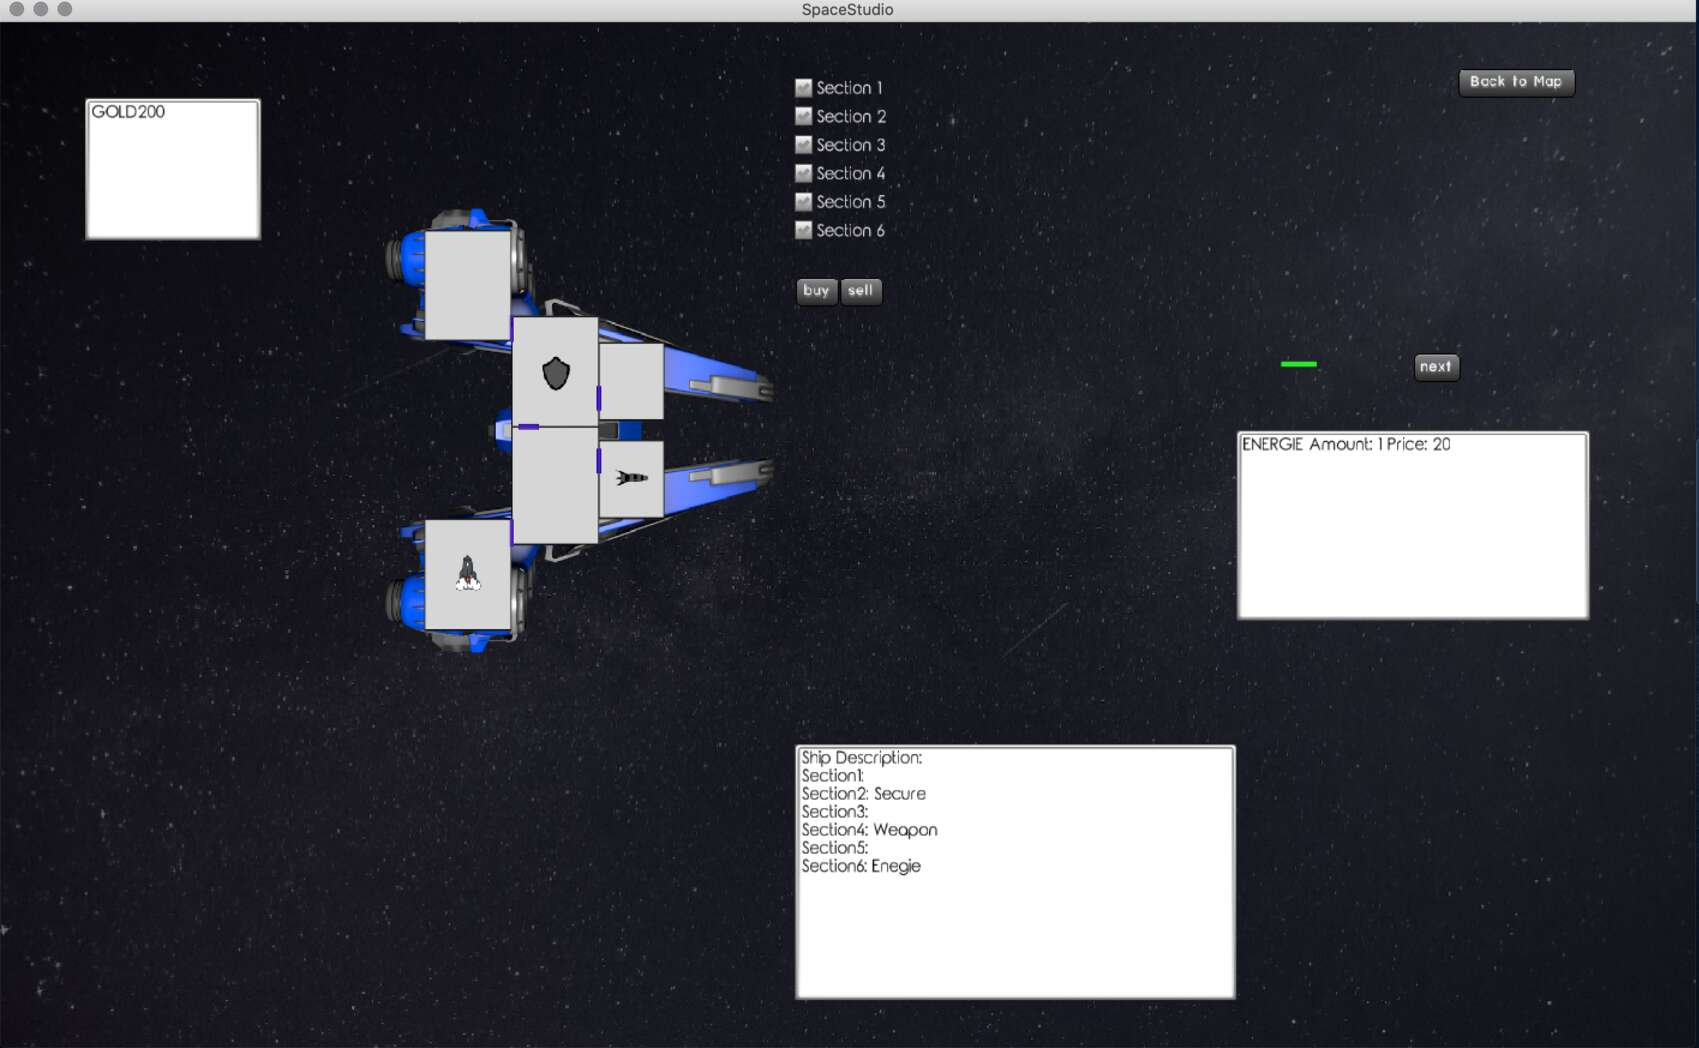
\includegraphics[scale=0.4]{TestProtocolBilder/energie.jpg}
\caption{andere Typ von Ereignisse}
\end{figure}
\newpage
\subsubsection{Waffen kaufen}
Der Kauf von Waffen wurde getestet, diese Aktion verringert das Gold des Spielers.\\
Eingabe: Der Spieler kauft Waffen.\\
Ergebnis: Das Raumschiff bekommt die gekaufte Waffe und kann diese im Combat-Screen verwenden.
\begin{figure}[htp]
\centering
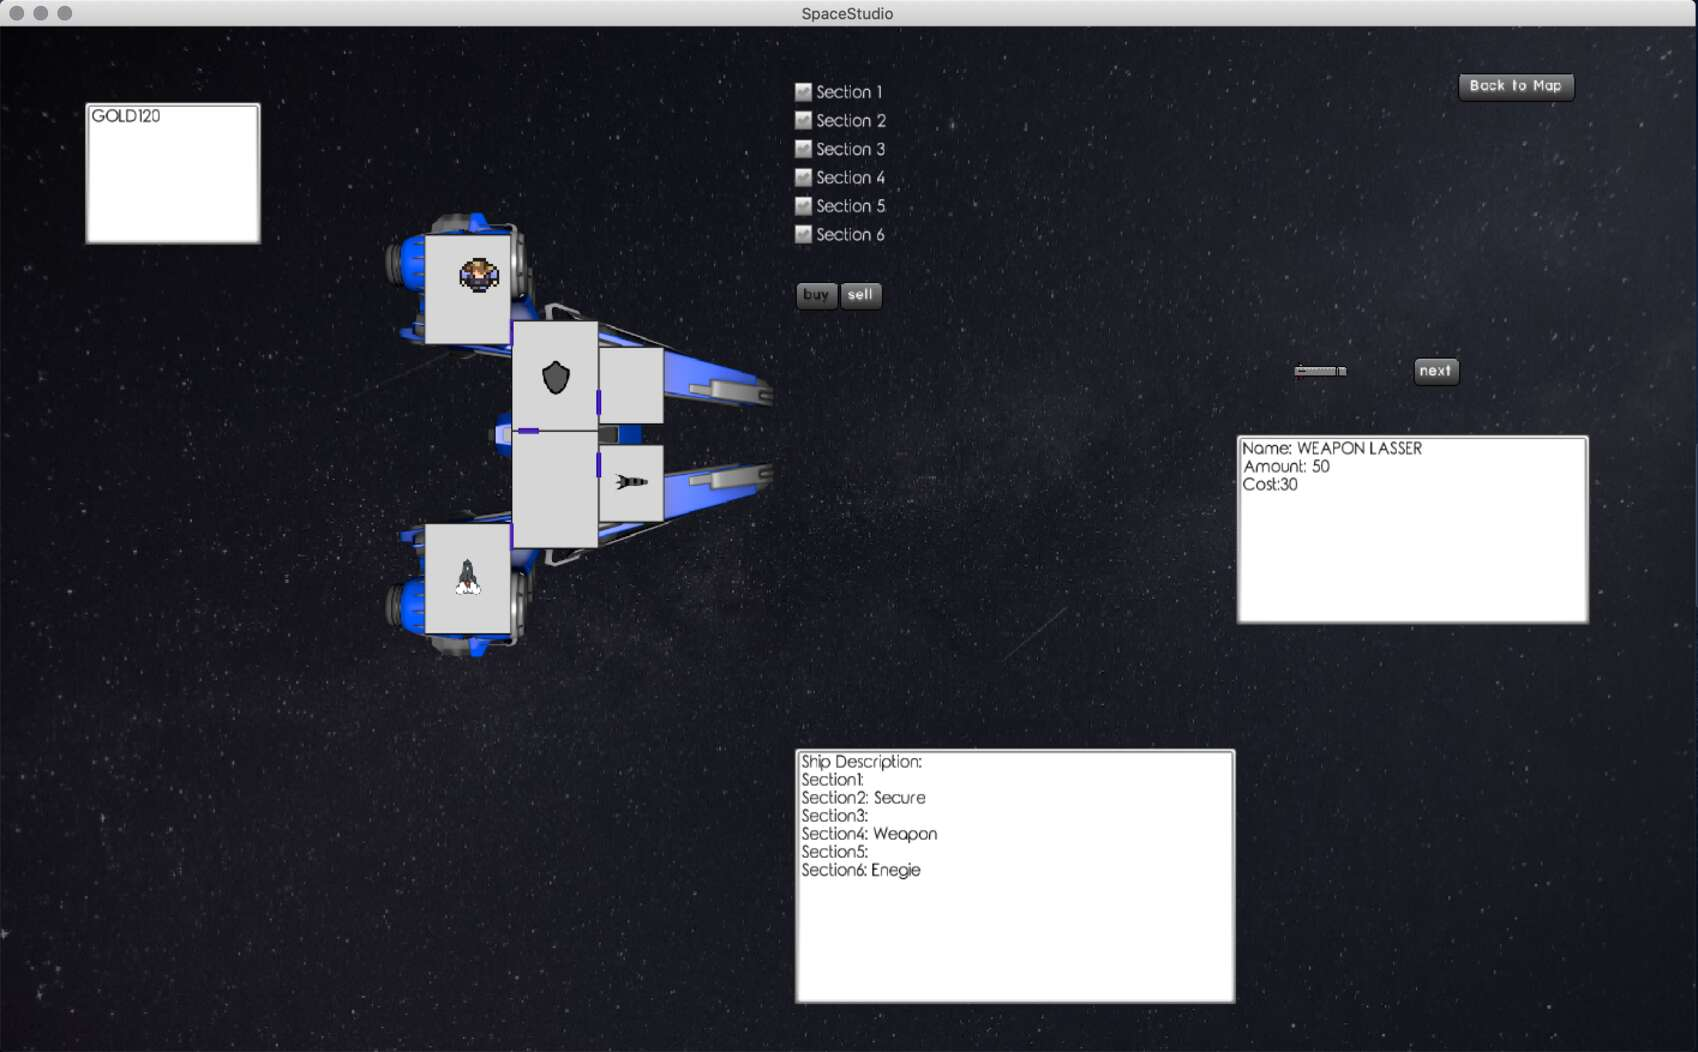
\includegraphics[scale=0.4]{TestProtocolBilder/weaponkaufen.jpg}
\caption{Anderer Typ von Ereignissen}
\end{figure}
\newpage
\subsubsection{Crewmember kaufen}
Beim Kauf von Mitgliedern wurde getestet, dass zuerst ein Abschnitt ausgewählt werden muss, in dem dieses Mitglied positioniert werden muss, wenn der Kauf getätigt werden kann.\\
Eingabe: Der Spieler kauft einen Crewmember und wählt die Sektion in der der Crewmember aufgestellt werden soll.\\
Ergebnis: Der Crewmember wird dem Raumschiff in die ausgewählte Sektion hingestellt.\\
\begin{figure}[htp]
\centering
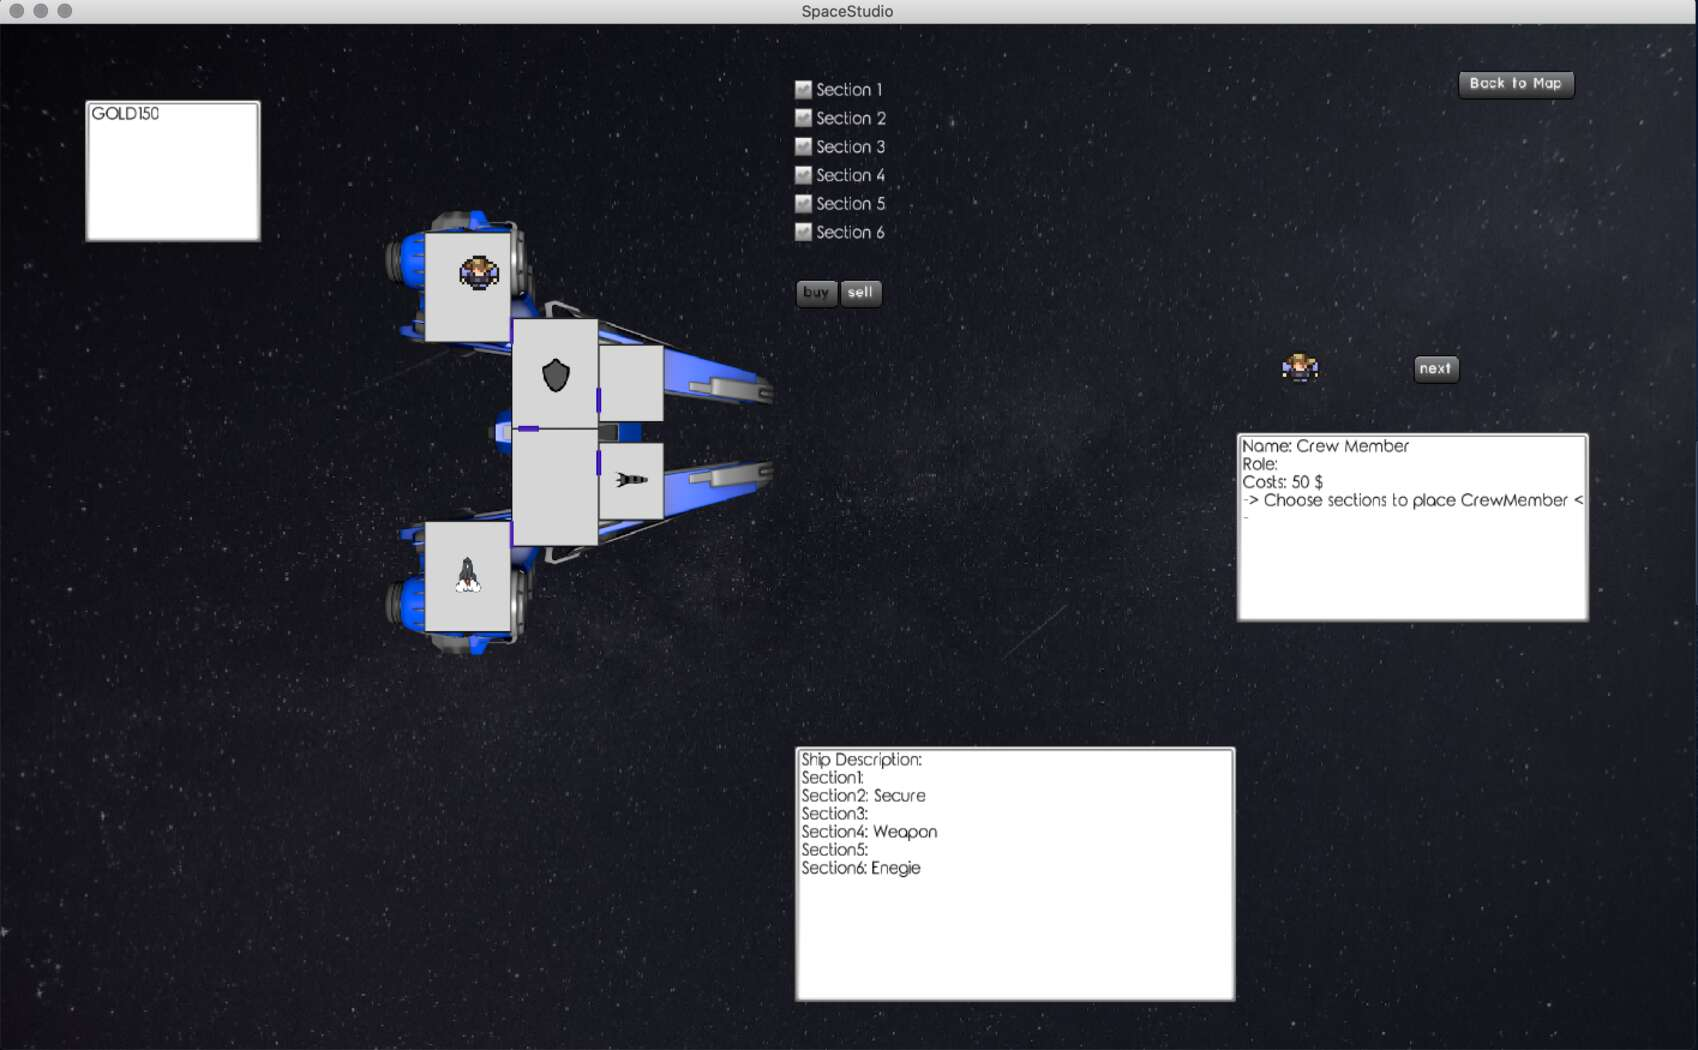
\includegraphics[scale=0.4]{TestProtocolBilder/crewmemberkaufen.jpg}
\caption{Anderer Typ von Ereignissen}
\end{figure}


\newpage
\section{Combat Screen}
Tested succesfully by Santiago Rey on 02.08\\\\
Auf diesem Bildschirm wird jeder Knopf getestet und die Logik für einen Kampf ermittelt.

\subsection{Initial Combat Screen}
Die Hauptschaltfläche auf dem Bildschirm ist der unterste Knopf, mit der Sie eine Runde starten oder beenden können. Dieser Button verringert das Aufwärmen und lässt Waffen schießen.\\
Eingabe: Der Spieler drückt den Knopf Waiting/Playing.\\
Ergebnis: Die Runde wird gestartet oder beendet. Entweder schießt der Spieler oder sein Gegner.\\
\begin{figure}[htp]
\centering
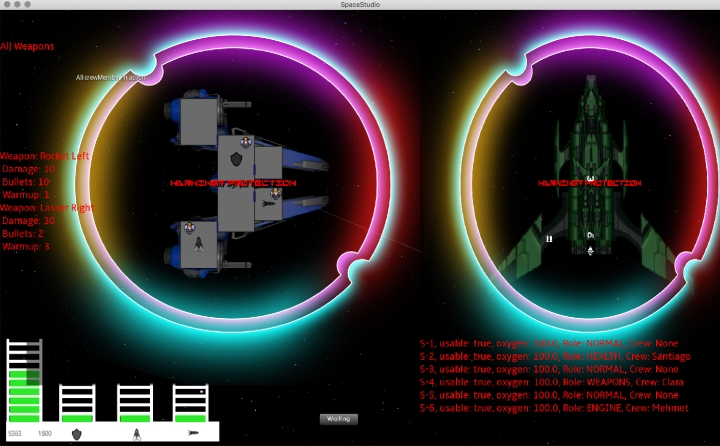
\includegraphics[scale=0.7]{TestProtocolBilder/OptimizedinitialBattelScreen.png}
\caption{Anderer Typ von Ereignissen}
\end{figure}

\newpage
\subsection{Energieverteilung}
Die Beschriftungen unten rechts ermöglichen es, den Zustand der Player zu kennen. Diese ändern sich dynamisch nach den Anweisungen des Spielers.\\
Ereignis: Der Spieler verteilt eine Energie an das System Waffen.\\
Ergebnis: Die Gesamtanzahl der Energie verringert sich um eins und die Anzahl der Energie, die das Waffensystem hat, wird um eins erhöht.\\
\begin{figure}[htp]
\centering
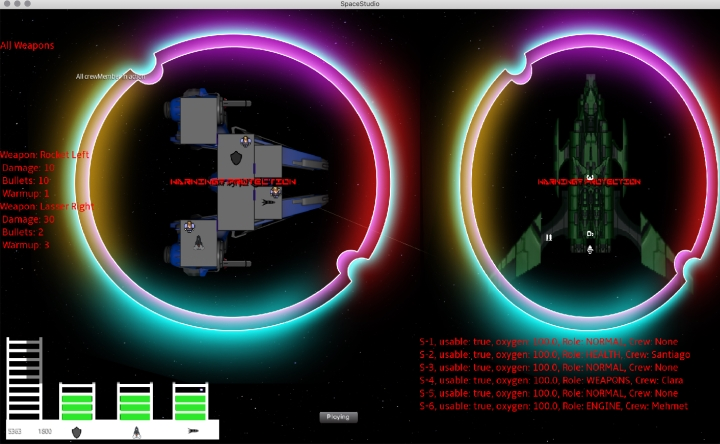
\includegraphics[scale=0.7]{TestProtocolBilder/OptimizedEnergieAlleSysteme.png}
\caption{Anderer Typ von Ereignissen}
\end{figure}

\newpage
\subsection{Keine Energie im Waffen System}
Jeder Knopf wurde getestet, um die Energie zu teilen, und es wurde getestet, dass das Waffensystem, wenn es keine Energie hat, nicht feuern kann.\\
Eingabe: Der Spieler reduziert die Energie vom Waffensystem auf null.\\
Ereignis: Der Spieler kann nicht mehr schießen, da das Waffensystem mindestens ein Energie haben muss um schießen zu können.\\
\begin{figure}[htp]
\centering
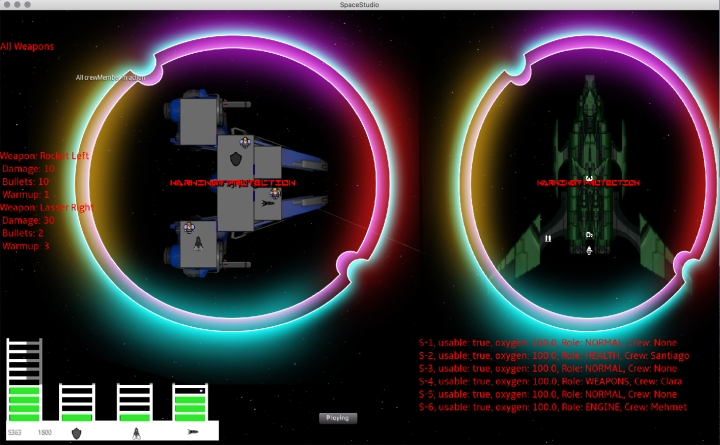
\includegraphics[scale=0.7]{TestProtocolBilder/OptimizedEnergieVerteilung.png}
\caption{Anderer Typ von Ereignissen}
\end{figure}

\newpage
\subsection{Gegner schießt}
Es wurde getestet, dass der Gegner, wenn er an der Reihe ist, schießen kann und die Kugeln in der grafischen Oberfläche gerendert werden.\\
Eingabe: Der Spieler beendet seine Runde und der Gegner ist dran.\\
Ergebnis: Der Gegner schießt auf eine beliebige Sektion. Das Schutzschild wird beschädigt.\\
\begin{figure}[htp]
\centering
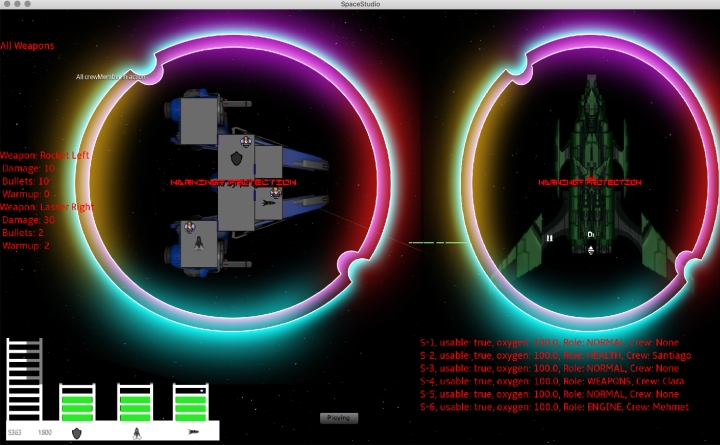
\includegraphics[scale=0.7]{TestProtocolBilder/OptimizedgegnerShots.png}
\caption{andere Typ von Ereignisse}
\end{figure}


\newpage
\subsection{Player schießt}
Es wurde auch getestet, dass der Benutzer feuern kann, sobald ein feindlicher Abschnitt ausgewählt wurde, dass das Aufwärmen Null ist und dass der Waffenabschnitt verwendbar ist. Auch, dass die Kugeln gerendert werden.\\
Eingabe: Der Spieler wählt ein System des Gegners aus und schießt auf diese mit der Leertaste.\\
Ergebnis: Das Schutzschild des Gegners wird beschädigt.\\
\begin{figure}[htp]
\centering
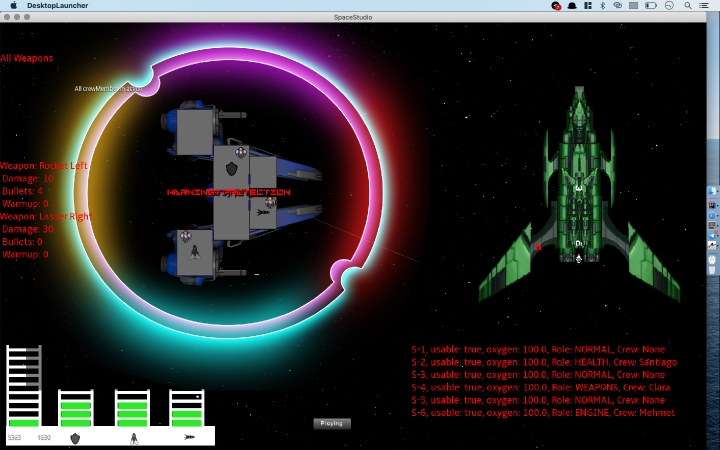
\includegraphics[scale=0.7]{TestProtocolBilder/OptimizedweaponsShot.png}
\caption{Waffen können wieder feuern, wenn das System eingeschaltet wurde.}
\end{figure}

\newpage
\subsection{Win Screen}
Es wurde getestet, dass der Benutzer beim Schießen des Spielers eine Verkürzung des Lebens des Gegners feststellen kann. Wenn das Leben des Gegners Null erreicht, wird der Benutzer gewarnt, dass er weiterhin Planeten erforschen kann.\\
Eingabe: Der Spieler greift den Gegner an und das gegnerische Raumschiff wird zerstört.\\
Ergebnis: Ein Dialog erscheint und der Spieler hat den Kampf gewonnen und kann zur Kartenansicht zurückkehren.\\
\begin{figure}[htp]
\centering
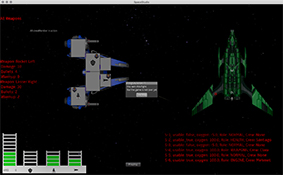
\includegraphics[scale=1.2]{TestProtocolBilder/wonScreen.jpg}
\caption{Win Screen, als der Feind besiegt wurde }
\end{figure}
\newpage
\subsection{Bewegung der Mitglieder}
Wenn ein Teammitglied aus dem Bereich verschoben wird, sehen Sie Symbole, wo dieses Teammitglied platziert werden kann.\\
Eingabe: Der Spieler bewegt ein Crewmitglied in eine andere Sektion.\\
Ergebnis: Es dauert eine Runde Zeit bis das Crewmitglied in die ausgewählte Sektion gelangt. Eine Sanduhr erscheint.\\
\begin{figure}[htp]
\centering
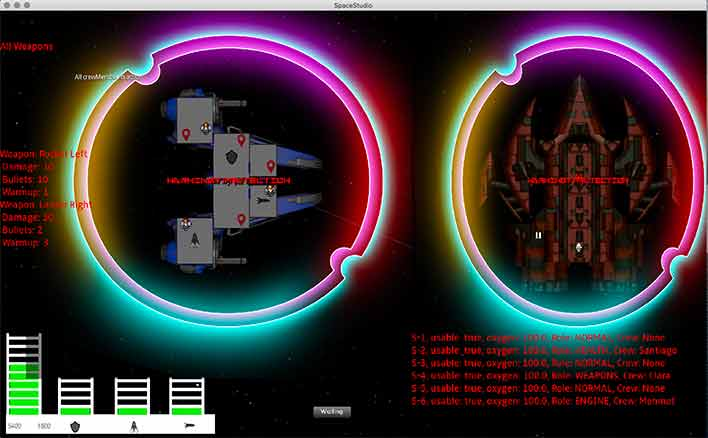
\includegraphics[scale=0.6]{TestProtocolBilder/crewmemberpull@0,25x.jpg}
\caption{Crewmember auf andere Sektionen bewegen}
\end{figure}
\newpage
\subsection{Wartezeit}
Es ist notwendig, einige Zeit zu warten, bis die Mitglieder, die geändert wurden, den Abschnitt erreichen. Deshalb ist das Sanduhrsymbol aufgesetzt. Diese Implementierung wurde erfolgreich getestet.
\begin{figure}[htp]
\centering
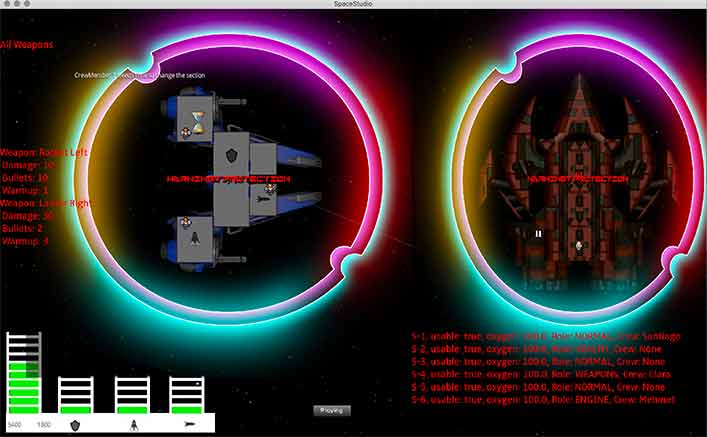
\includegraphics[scale=0.6]{TestProtocolBilder/timewaiting@0,25x.jpg}
\caption{Wartezeit für Crewmember Bewegungen}
\end{figure}
\newpage
\subsection{Crewmember sterben}
Crewmember können, wenn zu wenig Oxygen in der Sektion enthalten ist, auch sterben.\\
Eingabe: Der Gegner beschädigt eine vom Crewmember besetzte Sektion und das Oxygen in dieser Sektion sinkt.\\
Ergebnis: Der Crewmember in dieser Sektion stirbt. Dazu wird ein Dialog angezeigt mit dem Hinweis das der Crewmember gestorben ist.\\
\begin{figure}[htp]
	\centering
	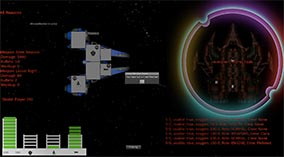
\includegraphics[scale=1.5]{TestProtocolBilder/crewMemberDead@0,25x.jpg}
	\caption{Crewmember können sterben}
\end{figure}
\newpage
\subsection{Dunkle Planeten}
Es wurde getestet, dass wenn der Benutzer vom Planeten springt, der besuchte Planet dunkel angezeigt wird, so dass der Benutzer weiß, welche Planeten er schon besucht hat.\\
Eingabe: Der Spieler besucht ein Planet und fliegt dann einen anderen Planeten.\\
Ergebnis: Der vorherige Planet wird dann als ein dunkler Planet angezeigt.\\
\begin{figure}[htp]
\centering
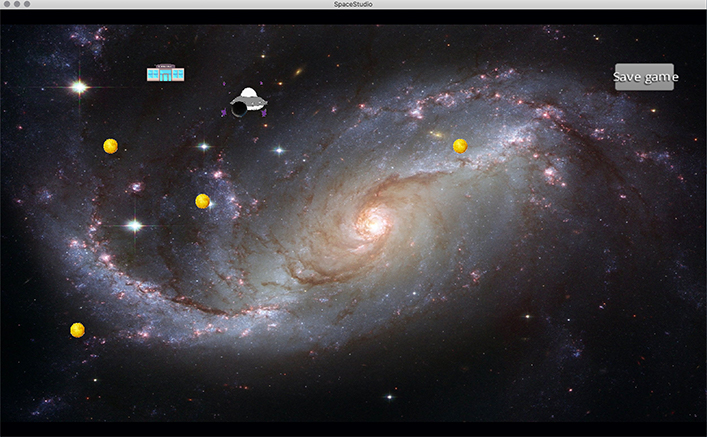
\includegraphics[scale=0.6]{TestProtocolBilder/besuchtePlanet.jpg}
\caption{Dunkle Planeten}
\end{figure}
\newpage
\subsection{Upgrade}
Wenn Sie auf die Schaltfläche Upgrade klicken, sehen Sie die möglichen Optionen zur Verbesserung des Schiffs des Spielers.\\
Eingabe: Nachdem ein Planet angeflogen wurde und drückt der Spieler auf Upgrade.\\
Ergebnis: Dem Spieler werden mehrere Upgrademöglichkeiten angezeigt.\\
\begin{figure}[htp]
\centering
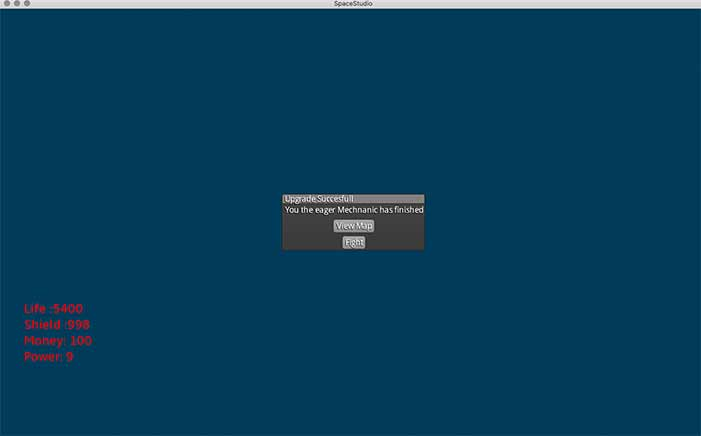
\includegraphics[scale=0.6]{TestProtocolBilder/nachupgrade@0,25x.jpg}
\caption{Upgrade Optionen}
\end{figure}

Wenn ein Upgrade ausgewählt wurde, können Sie mit dem Kampfbildschirm fortfahren.
\begin{figure}[htp]
\centering
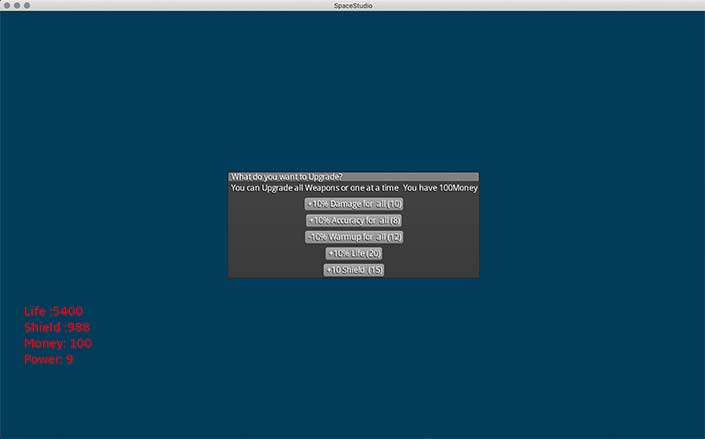
\includegraphics[scale=0.6]{TestProtocolBilder/upgrade@0,25x.jpg}
\caption{Nach Upgrade zum Combat Screen}
\end{figure}

\newpage
\section{Spiel speichern und fortsetzen}
Während des Spiels kann der Spieler das Spiel speichern um zu einem späteren Zeitpunkt das Spiel wieder aufzunehmen und fortzusetzen.\\
Eingabe: Der Spieler speichert seinen Spielstand ab.\\
Ergebnis: Der Spielstand wird in der Datenbank gespeichert.\\
\begin{figure}[htp]
	\centering
	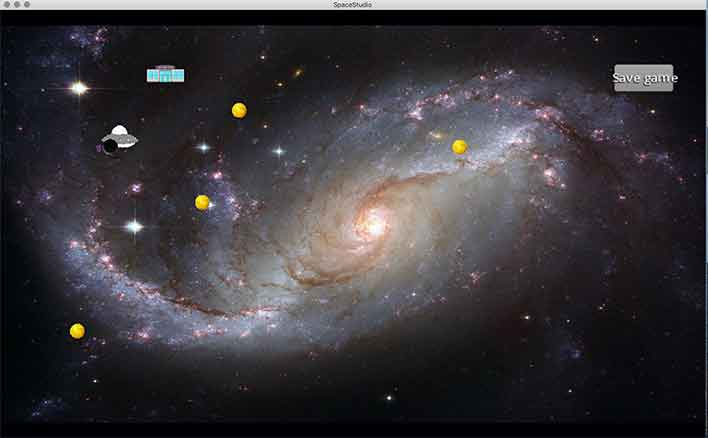
\includegraphics[scale=0.6]{TestProtocolBilder/continue1@0,25x.jpg}
	\caption{Spiel abbrechen und speichern}
\end{figure}

Mit dem "Save game" Button kann der Spieler das Spiel speichern.\\
\begin{figure}[htp]
	\centering
	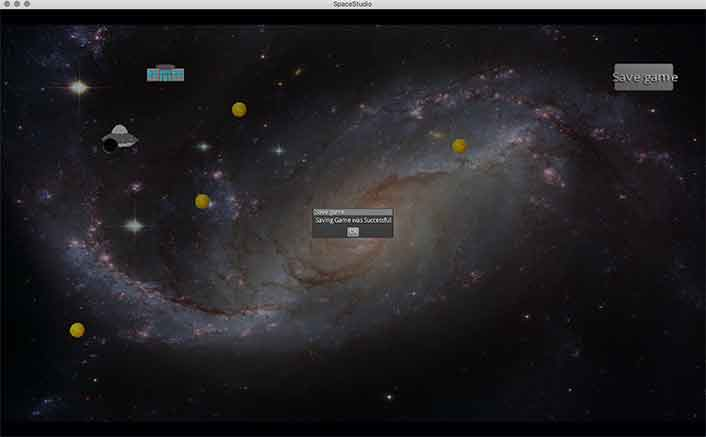
\includegraphics[scale=0.6]{TestProtocolBilder/save@0,25x.jpg}
	\caption{Spiel speichern Button}
\end{figure}
\clearpage
Der Spieler kann das Spiel zu einem späteren Zeitpunkt wieder aufnehmen und fortsetzen. Dafür muss der Spieler im Menü Screen den Button "Continue" drücken. Dann gelangt der Spieler zu seinem alten Spielstand zurück.\\
Eingabe: Der Spieler drückt auf den Button Continue.\\
Ergebnis: Der Spieler gelangt wieder zu seinem alten Spielstand und kann weiterspielen.\\
\begin{figure}[htp]
	\centering
	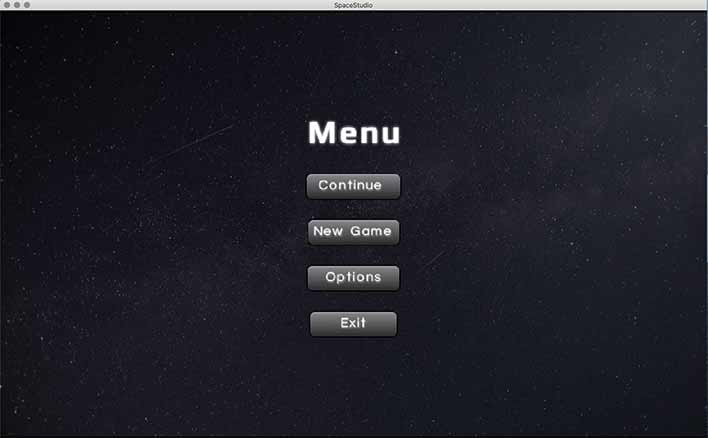
\includegraphics[scale=0.6]{TestProtocolBilder/continuebutton@0,25x.jpg}
	\caption{Das Spiel fortsetzen}
\end{figure}
\clearpage
Wenn der Spieler dann auf Continue drückt kommt er wieder auf den alten Spielstand zurück.
\begin{figure}[htp]
	\centering
	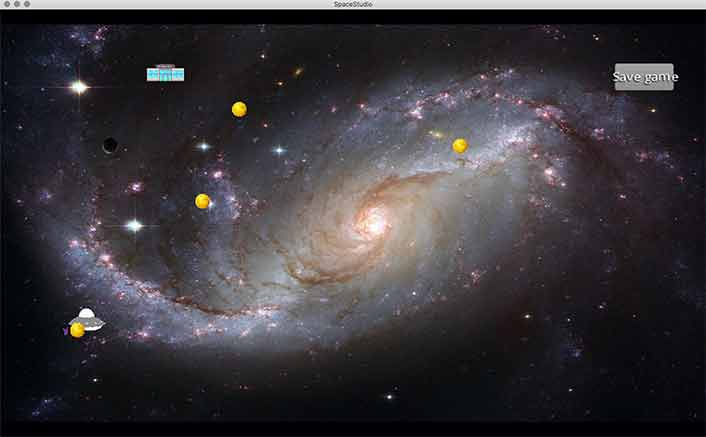
\includegraphics[scale=0.6]{TestProtocolBilder/continueScreen@0,25x.jpg}
	\caption{Alten Spielstand fortsetzen}
\end{figure}

\newpage
\section{Multiplayer}
Man kann auch gegen einen echten Spieler spielen. Dafür müssen die beide Spieler in den Multiplayer Modus gehen.\\
Eingabe: Beide Spieler drücken auf den Multiplayer Button\\
Ergebnis: Beide Spieler gelangen in den Ship-Select-Screen.\\
\begin{figure}[htp]
	\centering
	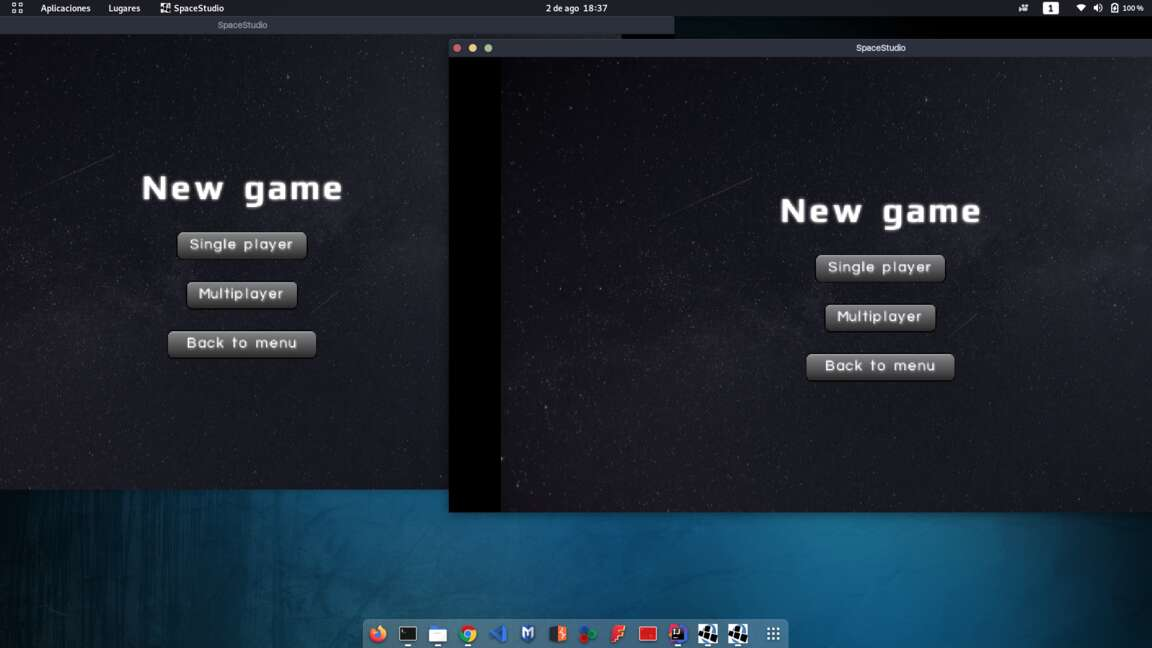
\includegraphics[scale=0.4]{TestProtocolBilder/Multiplayer/1.jpg}
	\caption{Multiplayer Menü Screen}
\end{figure}
\clearpage
Im Ship-Select-Screen wählen beide das Raumschiff aus und müssen den Ready-Up Button drücken um anfangen können.\\
Eingabe: Beide Spieler drücken auf Ready Up.\\
Ergebnis: Das Spiel beginnt und beide Spieler gelangen in die Kartenansicht.\\
\begin{figure}[htp]
	\centering
	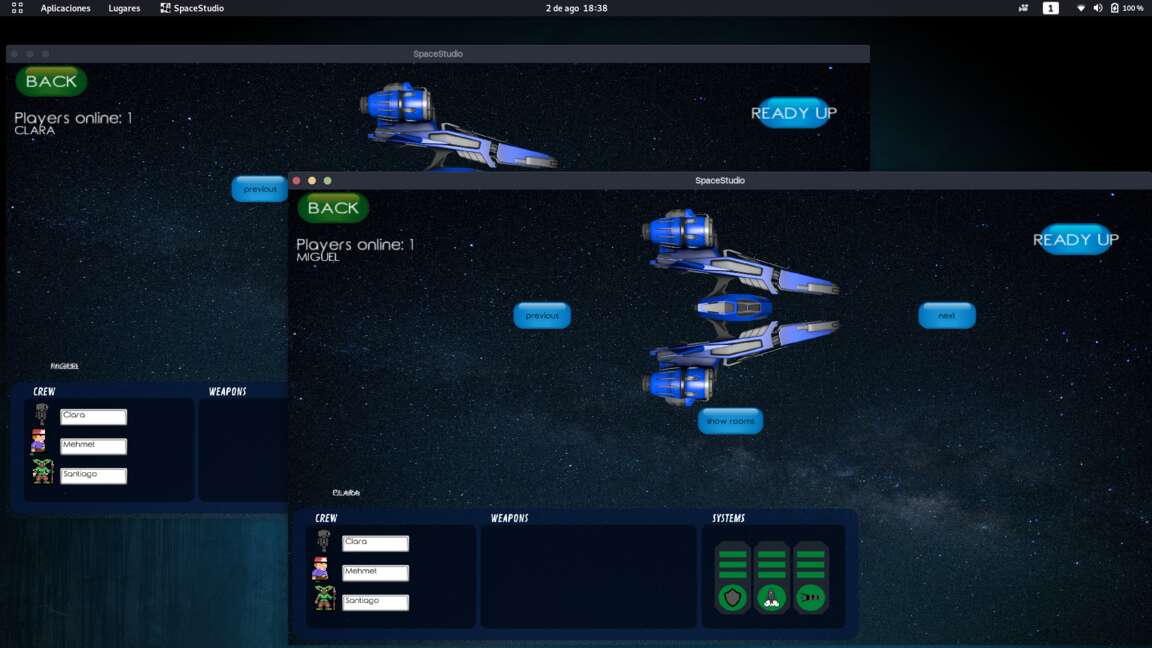
\includegraphics[scale=0.4]{TestProtocolBilder/Multiplayer/2.jpg}
	\caption{Multiplayer Synchronisierung}
\end{figure}
\begin{figure}[htp]
	\centering
	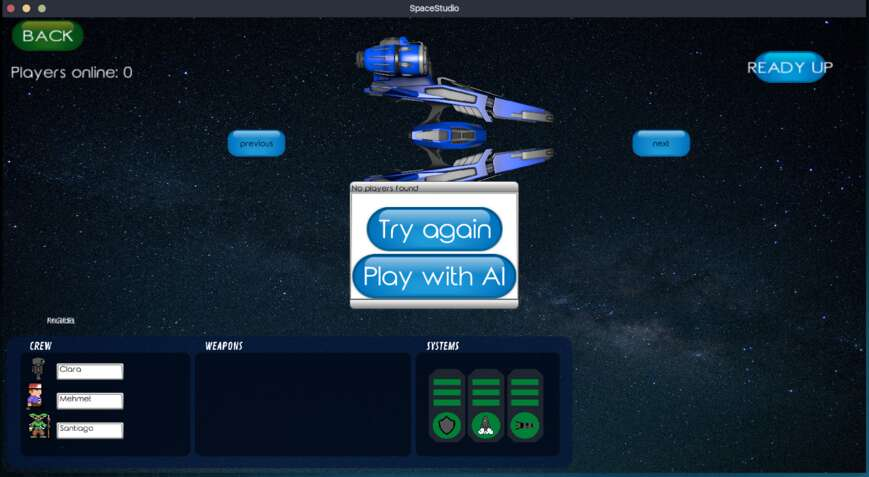
\includegraphics[scale=0.48]{TestProtocolBilder/Multiplayer/3.jpg}
	\caption{Wartet auf die Antwort des Servers}
\end{figure}
\begin{figure}[htp]
	\centering
	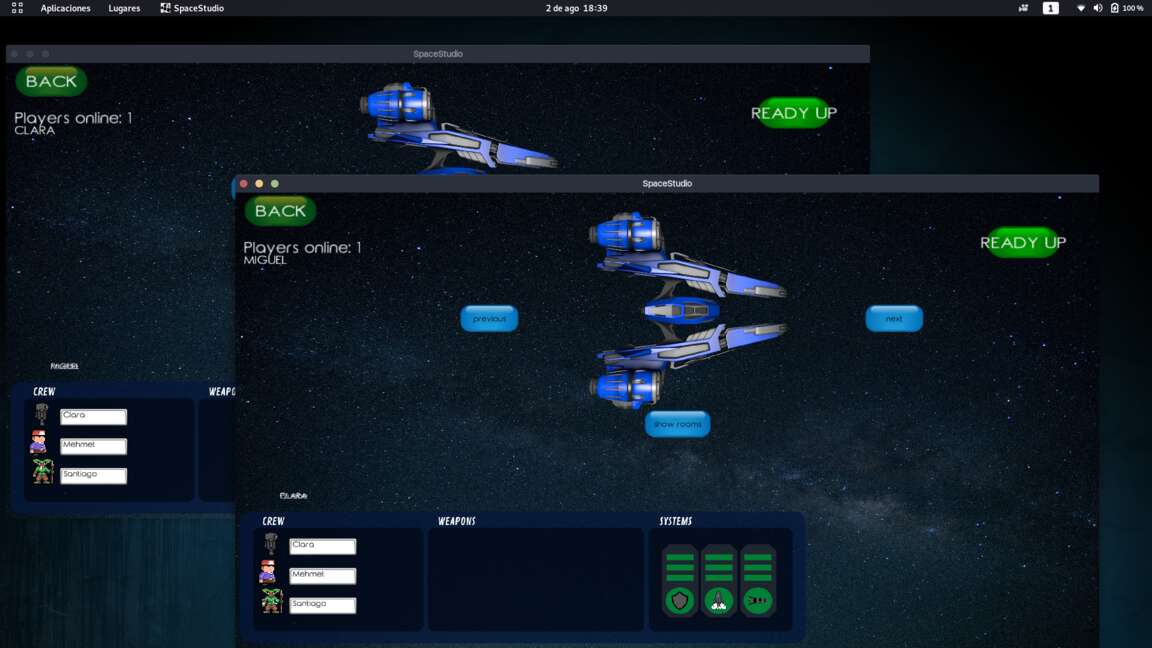
\includegraphics[scale=0.4]{TestProtocolBilder/Multiplayer/4.jpg}
	\caption{Multiplayer Synchronisierung erfolgreich}
\end{figure}
\end{document}

